%!TEX root = ../thesis.tex

\thispagestyle{myheadings}

\graphicspath{{Body/Figures/Wa/Temporary/}{Body/Figures/Wa/Temporary/FitResiduals/}{Body/Figures/Wa/Reconstruction/}{Body/Figures/Wa/Histogramming/}{Body/Figures/Wa/Pileup/}{Body/Figures/Wa/Pileup/TimeAndEnergySpectra/}{Body/Figures/Wa/Pileup/Scaling/}{Body/Figures/Wa/RatioAnalysis/}{Body/Figures/Wa/RatioAnalysis/MethodOverview/}{Body/Figures/Wa/RatioAnalysis/VW_Studies/}{Body/Figures/Wa/Datasets/9d/EnergyThreshold/}{Body/Figures/Wa/Datasets/Endgame/LostMuonFiles/MainCuts/}{Body/Figures/Wa/Datasets/ComparisonPlots/LostMuons/}}

\chapter{\texorpdfstring{\wa}{wa} Measurement}
\label{chapter:wa}


The measurement of \wa is determined by counting the number of detected positrons in the calorimeters above some energy threshold, as described in \secref{section:WaIntro}. Doing so results in a histogram of counts which is modulated by \wa, \figref{fig:gm2wiggle}. Fitting for the frequency allows \wa to be extracted. The \wa measurement therefore consists of the steps needed to construct the histogram of counts, the fitting of that histogram, and any systematic studies done in the analysis. 


\section{Reconstruction of decay positron hits}
\label{sec:ReconWest}


The calorimeters measure hit times and energies of impacting particles, where these hit times and energies are determined from the raw SiPM signals and a reconstruction procedure. In E989 there are two overall separate reconstruction algorithms, \texttt{ReconWest} and \texttt{ReconEast}, both written in the \textit{art} framework similar to the tracking reconstruction. Each of these reconstruction algorithms is modularized, and the steps of the reconstruction process can be switched in and out at will. Using separate reconstruction methods gives confidence in any final results by removing single points of failure. The reconstruction method used in this analysis is \texttt{ReconWest}. A summary of its details will be presented here. A more thorough description is detailed by A. Fienberg \cite{AFThesis}.


The raw data are digitized waveforms, which are voltage versus time traces output from each SiPM for each calorimeter crystal hit. Due to the incredible amount of data coming in with the high muon fill rate, only those pulses which exceed some threshold are saved to disk. An online processing system checks the traces against this pre-configured threshold by passing all of the data through a GPU farm \cite{Gohn:2016shi}. If any trace is found above threshold, then the data is saved from every SiPM in every calorimeter, for a time range around the over-threshold trace. This time range is called a time island, similar to that in the tracking reconstruction, and typically has a width of $\SI{40}{ns}$ \cite{AFThesis}.


The traces are then fit with templates in order to extract the the area and peak times of any present pulses. Each SiPM has its own templates, one for positrons and one for laser pulses. These templates are extracted from data, where each template is determined by collecting many single pulse traces from a SiPM, normalizing by pulse area, aligning in time, and averaging them. These templates were checked against many systematic effects in order to make sure that the constructed templates did not bias the energy or time measurements, such as hit angle, energy (pulse size), position, and rate, as well as aging effects \cite{Kaspar:2016ofv,AFThesis}. Each trace is fit using a \chisq minimization algorithm with the corresponding SiPM templates in order to determine the time and energy of the hit. In order to fit for multiple pulses in a single time island, the fitting procedure first fits with a single template, and then checks the residuals for any remaining peaks. If peaks exist above some threshold, then the fitting is repeated until all pulses have been fit. The time measurement performance in the pulse finding was found to be unaffected by the number of pulses in a time island, and there is 100\% pileup separation at \ns{5} \cite{AFThesis}. See \figref{fig:TemplateFit} for a typical single template fit to a SiPM trace.


\begin{figure}[]
    \centering
    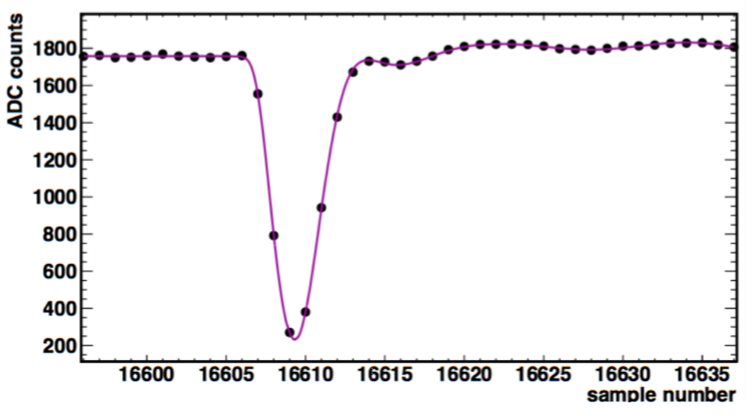
\includegraphics[width=0.6\textwidth]{TemplateFit}
    \caption[Template fit to SiPM trace]{A template fit in purple to a SiPM trace delineated by the black points which is in units of ADC counts. Plot courtesy of Aaron Fienberg.}
    \label{fig:TemplateFit}
\end{figure}


Once a pulse has been fit with a template, the pulse area needs to be converted to real energy units using an energy calibration procedure. A couple of different techniques exist that can be used, including a method that counts photo-statistics seen in the SiPMs \cite{AFThesis}. The default method used is a comparison of lost muon energy signatures in the calorimeters. As described in \refref{lostmuons}, muons lost from the storage ring can spiral inward and hit consecutive calorimeters with a specific time separation between calorimeter hits. These lost muons are minimum-ionizing particles, and thus leave a very distinct energy signature in the crystals, see \secref{sec:lostmuons}. Selecting on the time signature allows hits corresponding to lost muons to be isolated, and the energy signature can be used to determine the appropriate conversions from area to energy\footnote{Different channels can also be equalized based on the energy signatures.}. 


The energy calibration for positron hits as compared to lost muon hits then needs to be determined. Again there are a couple of different techniques, including a comparison of endpoint energies for high energy positrons which tail off at the magic momentum of $\SI{3.094}{\GeV}$, and comparison with simulation. The default technique is to calibrate the energies such that the optimal energy threshold for the \wa analysis is near $\SI{1.7}{\GeV}$ \cite{AFThesis}. Ultimately the energy calibration doesn't matter too much because it is not the energy units that really matter. What really matters is the number of positrons above some energy threshold, where that threshold can be optimized empirically. In fact, the entire \wa analysis could be done without even considering the energy of the incident positrons, and only considering the area of the SiPM pulses\footnote{This statement ignores the effects of pileup which must be accounted for, and applies for a threshold style analysis, and not for other analysis methods which depend on the energy of the pulses.}.


Each pulse fit now has an associated energy and time. Because the measurement of \wa depends heavily on the time reconstruction since the analysis is a frequency extraction, pulse times need to be corrected for various effects in order to reach the precision goal. The fitted times for each pulse need to be aligned on a fill-by-fill basis relative to the injection time of the beam, corrected for any channel differences due to differing pulse shapes or fiber lengths, and corrected for any calorimeter time misalignments due to the use of different laser system components. The fill-by-fill alignment is corrected for using the T0 detector as described in \secref{sec:T0}. The channel differences are corrected by aligning calorimeter channels in time using signals from islands with large simultaneous pulses in neighboring crystals. Calorimeters are time aligned using lost muon coincident events as described before. Once the times of the pulse fits or crystal hits have been determined, the energies can be corrected appropriately for gain effects measured by the laser system. As described in \secref{sub:LaserCalibrationSystem}, the laser calibration system corrects for in-fill, out-of-fill, and SDTP effects \cite{Gain}. \figref{fig:IFGFunction} shows an in-fill gain function fit to data for a single calorimeter. Systematic effects for corrected gain effects are studied in \secref{sub:gainerror}. 

\begin{figure}[]
    \centering
    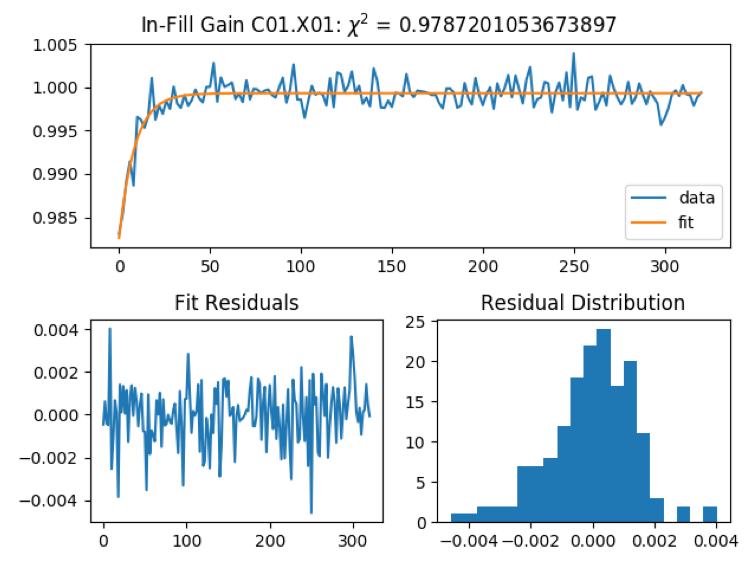
\includegraphics[width=0.6\textwidth]{IFGFunction}
    \caption[In-fill gain function fit for a single calorimeter crystal]{In-fill gain function fit for a single calorimeter crystal (top) and fit residuals (bottom). Each crystal has its own in-fill and SDTP gain function parameters. Plot courtesy of Matthias Smith.}
    \label{fig:IFGFunction}
\end{figure}


The last part of the calorimeter reconstruction is the clustering. Clustering is the stage which takes the individual template fit results from separate crystals, and turns them into the times, energies, and positions of decay positron impacts. For a time island with a single positron impact, the procedure is straightforward. The energy for the positron hit cluster is the sum of the individual hit crystal energies. The time for the cluster is taken as the time of the maximum energy hit in the island. This works because most of the deposited energy from a hit is localized to a single crystal. The position of the cluster is determined with a logarithmic weighting function between crystal hits, which for a $\SI{2}{\GeV}$ positron in the E989 calorimeters results in a resolution of $\SI{2}{mm}$ \cite{AFThesis}. See \figref{fig:CaloCluster} for a single calorimeter cluster from a positron hit in the calorimeter. For a time island with multiple positron impacts, the individual crystal hits are separated in time, where the time partitioning separates hits that are $\SI{2.5}{ns}$ apart, and the clustering proceeds as before. For hits which are within this time window, a pileup event has occurred. If the pileup event happens within the same crystal, then the multiple hits are measured as a single hit, and this needs to be corrected for using a pileup subtraction technique, as described in \secref{sub:pileupsubtraction}. For hits that occur in separate crystals, the pileup can be resolved using the spatial separation of the calorimeters. This is an ongoing area of work, and one technique is described in \refref{AFThesis}. For this analysis the spatial separation was turned off, which simplifies the analysis somewhat. This increases the amount of pileup seen in the data, which then needs to be handled by the pileup subtraction technique. For the precision of the Run 1 analysis result, this was found to be acceptable. 


\begin{figure}[]
    \centering
    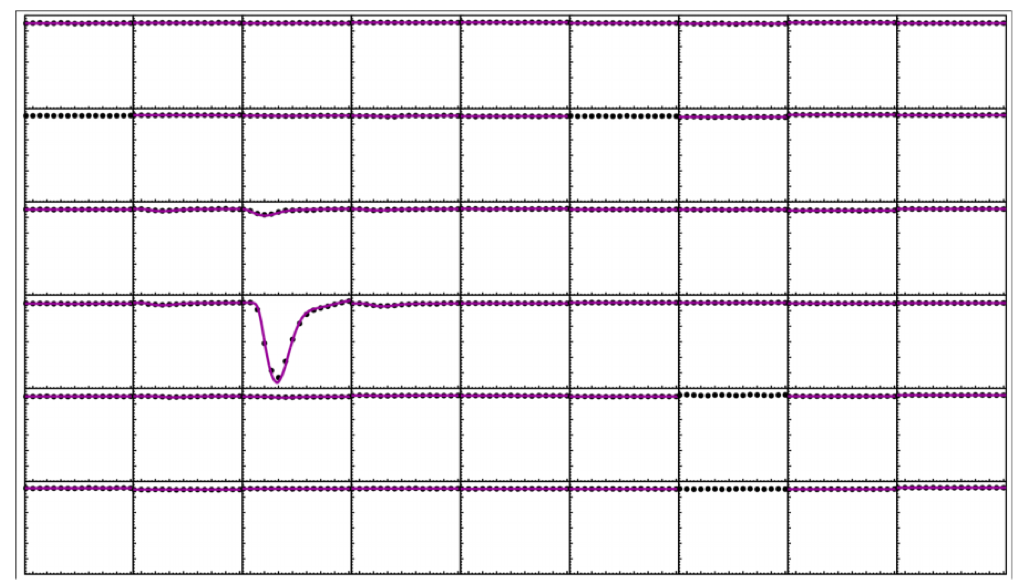
\includegraphics[width=0.9\textwidth]{CaloCluster}
    \caption[Calorimeter cluster from SiPM traces fit with templates]{A single positron hit in the calorimeter, which resulted in a reconstructed calorimeter cluster. Each box is a crystal in the calorimeter, where the contained trace is the SiPM output fit with a template. The positron hit the crystal three from the left and three from the bottom, where it deposited most of its energy. Some of the energy was deposited in the neighboring crystals. Plot courtesy of Aaron Fienberg.}
    \label{fig:CaloCluster}
\end{figure}



\section{Construction of positron hit energy and time spectra}
\label{sec:Histogramming}


Once the reconstruction has processed all calorimeter hits into clusters, the energy and time spectra histograms are made. At the very last stage of the reconstruction procedure, an \textit{art} module takes the produced clusters and puts them into \ROOT \texttt{TTree} formats, where individual data members include the energies, times, calorimeter numbers, etc. of the individual clusters. There is of order 20,000--140,000 cluster data files per dataset, which are combined down to order 200--1,400 \ROOT \texttt{TTree} files. These \ROOT \texttt{TTree}s are then passed through a \ROOT macro to produce \ROOT files with the histograms defined by the \texttt{TH1F} class, one \ROOT histogram file per tree file.


It should be noted that some of the parameter choices for the constructed histograms were informed by analysis results. All analysis parameters were chosen to be identical between the distinct analyzed datasets, in order to simplify both the comparison and combination of different dataset results. This section describes the justification for the different histogram parameters chosen. A table of the histogram parameters is shown in \tabref{tab:histogramparameters}.


\begin{table}[]
\centering
\setlength\tabcolsep{10pt}
\renewcommand{\arraystretch}{1.2}
\begin{tabular*}{.8\linewidth}{@{\extracolsep{\fill}}lc}
  \hline
    \multicolumn{2}{c}{\textbf{Time Spectra Parameters}} \\
  \hline\hline
    Parameter & Value \\
  \hline
    Energy threshold $(E_{th})$ & $\SI{1700}{\MeV}$ \\
    Bin width $(T_{c})$ & $\SI{149.2}{ns}$ \\
    Artifical dead time (ADT) & $\SI{5}{ns}$ \\
    Shadow dead time (SDT) & $\SI{5}{ns}$ \\
    Shadow gap time (SGT) & $\SI{10}{ns}$ \\
    Pileup energy scaling (C) & $1$ \\
    \gmtwo period $(T_{a})$ in Ratio Method & \mus{4.365411} \\
    Muon lifetime (\taumu) in Ratio Method & \mus{64.44} \\
  \hline 
\end{tabular*}
\caption[Parameters used in the construction of \wa time spectra]{Parameters used in the construction of \wa time spectra. \textbf{fill this table out more once I've gone through the various parts}}
\label{tab:histogramparameters}
\end{table}


Energy and time histograms are made for each individual calorimeter. These are summed together to form histograms of all hit times and energies. \figref{fig:energyHist} shows a sample energy spectrum for the Endgame dataset. An energy threshold is applied to the clusters before filling the time histograms. As described at the end of \secref{section:WaIntro}, the optimal energy threshold is where the quantity $NA^{2}$ reaches the maximum, at least in the case of a five parameter fit\footnote{Using the final fit function and looking at the error directly on the fitted \wa frequency, a slightly better estimate can be found.}. By scanning over the choice of energy threshold and fitting the resulting time spectra with \equref{eq:5parfunc}, the optimal energy threshold can be determined as seen in \figref{fig:OptimalEnergyThreshold}. The optimal choice of energy threshold was determined to be $\SI{1700}{\MeV}$, in accordance with the cluster reconstruction energy calibration. 

\begin{figure}[]
    \centering
    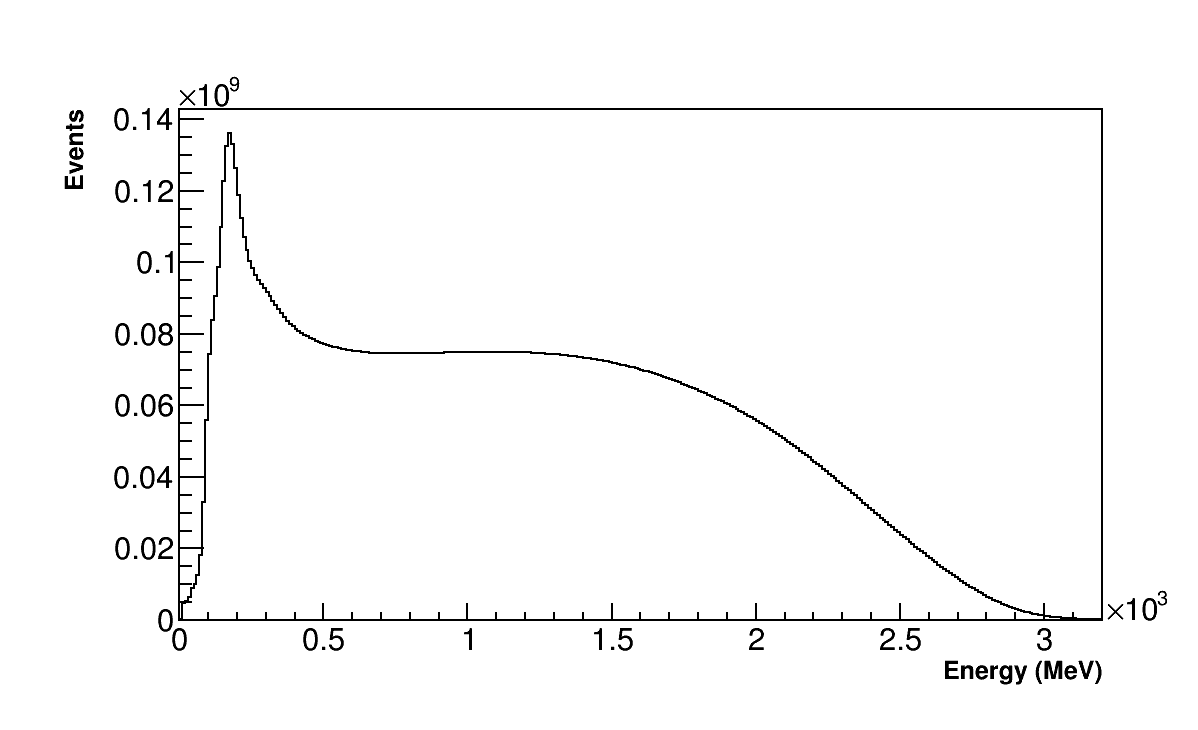
\includegraphics[width=0.7\textwidth]{basicEnergyHist}
    \caption[Sample energy spectrum]{Energy spectrum for hits in all calorimeters for the Endgame dataset on a linear scale. The peak at about 170 \MeV corresponds to lost muons.}
    \label{fig:energyHist}
\end{figure}


    \begin{figure}[]
    \centering
        \begin{subfigure}[t]{0.45\textwidth}
            \centering
            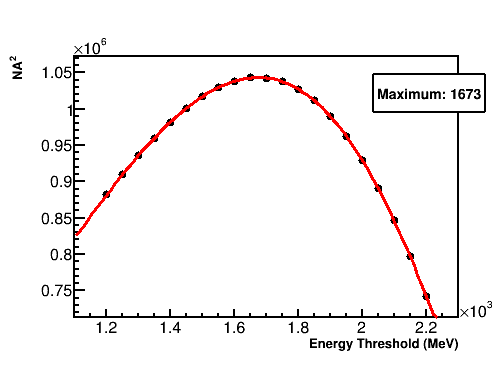
\includegraphics[width=\textwidth]{FiveParameter_NAsq_Vs_ETh_9d}
            \caption{}
        \end{subfigure}
        \begin{subfigure}[t]{0.45\textwidth}
            \centering
            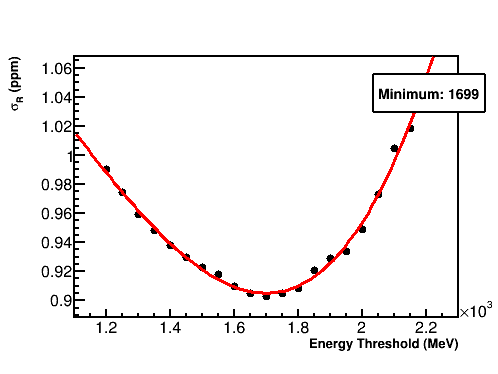
\includegraphics[width=\textwidth]{FullRatio_sigmaR_Vs_ETh_9d}
            \caption{}
        \end{subfigure}% 
    \caption[Determination of optimal energy threshold]{The optimal energy threshold can be determined from the $NA^{2}$ quantity as described in \secref{section:WaIntro} from five parameter fits to the data (left), or from the calculated error with the final fit function (right). The maximum and minimum are determined using seven parameter polynomial fits to the relevant quantities. The optimal threshold varies slightly per calorimeter and per dataset. Since the region of the minimum is flat, a single energy threshold of 1700 \MeV was chosen. These plots come from analyses to the 9d dataset.}
    \label{fig:OptimalEnergyThreshold}
    \end{figure}


The optimal bin width for the time histograms was determined to be $\SI{149.2}{ns}$, the average of the cyclotron periods determined from a fast rotation analysis to the data \cite{fastrotationsomething}. As described in \secref{sub:beam_debunching}, this bin width combined with a time randomization on each cluster over a range of $\pm T_{c}/2 = \SI{149.2}{ns} / 2$ serves to eliminate the fast rotation signal in the data\footnote{Some analyzers randomize all times in a single fill by half the cyclotron period as opposed to each individual pulse.}. This randomization is done using \ROOT's \texttt{TRandom3} class. As will be described in \secref{sub:vw_term}, the cluster times are also randomized by $\pm T_{VW}/2$, where $T_{VW}$ is determined per dataset. This is done in order to remove the effects of the VW in the data. \textbf{Should I put the actual numbers here? Need to look them up again.} The default random seed for each histogram \ROOT file is the hash of the input file name using C++'s standard hash class. Histograms are defined with a time range of 0--\mus{699.8972} (the closest integer multiple of the bin width to \mus{700}), corresponding to 4691 bins. Clusters with times less than \mus{25} or greater than \mus{660} are dropped, corresponding to 4256 bins containing data.



\subsection{Pileup subtraction}
\label{sub:pileupsubtraction}


As described in \secref{sec:Calorimeters}, there will be a certain amount of pileup in the detectors. Pileup again is the term for when multiple particles hit a calorimeter within the dead time of the detector such that they are registered as a single hit or cluster. The measured energy and time spectra for all observed clusters will include this pileup background. For the energy threshold time histogram, the number of counts will be wrong for cases where two below-threshold particles are registered as a single cluster above threshold, and where two above-energy threshold particles are registered as a single cluster. In the former, an extra count is added into the histogram, and in the latter a count is missed. The case where two lower energy positrons are registered as a single higher energy cluster will have a different \gmtwo phase than an actual single cluster at the same energy. This is because the lower energy positrons on average decay from muons which have travelled further around the ring, due to acceptance effects. These muons which have travelled further around the ring have spent more time in the magnetic field, and thus their spins have precessed more. See \figref{fig:PileupExample}. Clusters which originate from pileup events therefore have a different \gmtwo phase than non-pileup events. 


If pileup was a constant effect, then the phase of the time histogram would be shifted by some constant amount, and the extracted \wa frequency would be unaffected. However, the rate of pileup in the detectors changes over the time of a fill, as muons decay away. The rate of double pileup events in the detectors, where the word double indicates cases where two hits are registered as a single cluster, will go approximately as half the rate of single hit events\footnote{It is not exactly half when including the non-linear dead time of the detectors}, and similarly for triple and higher orders of the pileup effect. Because the rate of hits in the detectors oscillates at the \gmtwo frequency, pileup will increase and decrease accordingly leading to oscillations in the pileup time spectra at \wa and 2\wa. The lifetime of the overall pileup effect is approximately half the lifetime at which clusters are registered in the detectors, at \taumu, since double pileup is the dominant contribution. In order to to extract the correct \wa frequency, the pileup effect thus needs to be included in the fit function or subtracted out of the data. The former is challenging due to the non-linear nature of the dead time of the detectors, and would in the end include another phase in the argument of the cosine term in the fit function, thus worsening the statistical precision of the extracted \wa frequency. All analyzers thus construct an approximation of the pileup effect and subtract it from the data before fitting.


% -need to mention the \% level effect of pileup - ~1\% but where do you get that number...


\begin{figure}[]
    \centering
    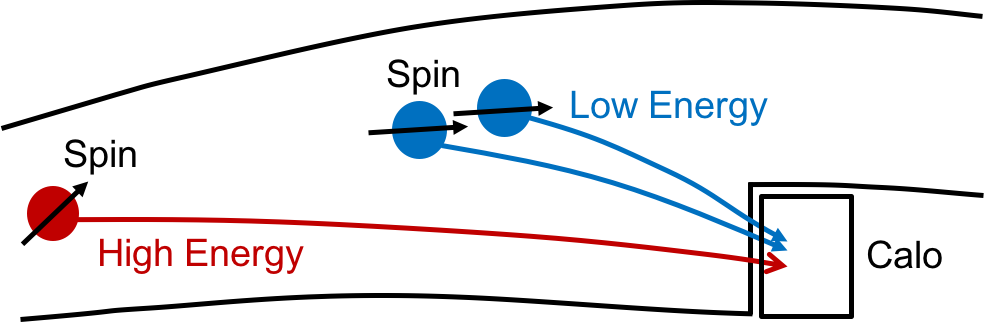
\includegraphics[width=0.5\textwidth]{PileupExample}
    \caption[Pileup example]{Pileup example, where two low energy positrons are registered as a single high energy positron. The black arrows indicate the (exaggerated) direction of the muon spins at the time of decay. Because of acceptance effects the lower energy decay positrons typically come from muons which have traveled further around the ring, and thus the muon spins have precessed more in the magnetic field, leading to a different measured \gmtwo phase for pileup events.}
    \label{fig:PileupExample}
\end{figure}


There are various methods to construct pileup spectra which are then subtracted off the main time and energy spectra. The method used in this analysis is called the `asymmetric shadow method', originally developed in E821 \cite{E821PileupShadow}. This method statistically constructs an approximation for the pileup from the data by assuming that the probability of observing a pileup pulse is the same as the probabilty that two pulses will be offset by some small amount of time, such as \ns{10}. The method works by looking in time windows after trigger pulses to see if a `shadow' pulse exists. If such a pulse exists, then a shadow doublet is created, see \figref{fig:ShadowPileupMethod}. The width of the time window, and the time offset from the trigger pulse to the window, are called the shadow dead time (SDT) and shadow gap time (SGT) respectively. The times and energies of the constructed pileup doublets are taken as
            \begin{gather}
                E_{\text{doublet}} = C \cdot (E_{1} + E_{2}), \label{eq:Edoublet} \\
                t_{\text{doublet}} = \frac{t_{1} \cdot E_{1} + (t_{2}-SGT) \cdot E_{2}}{E_{1} + E_{2}}, \label{eq:tdoublet}
            \end{gather}
where the energy of the doublet is the sum of the two singlet pulses $E_{1,2}$ times some calibration constant $C$, with a default value of 1, and the time of the doublet is the energy-weighted time of the two singlets $t_{1,2}$. The procedure for constructing the pileup spectra is as follows:
\begin{itemize}
    \item{Put each hit into a vector corresponding to a specific fill and a specific calorimeter}
    \item{Time order the hits}
    \item{Loop through the hits, for each hit look within a window of width SDT a time SGT later to see if a shadow pulse exists}
    \item{If a shadow pulse exists, construct a shadow doublet with energies and times as defined in Equations~\ref{eq:Edoublet} and \ref{eq:tdoublet}}
    \item{Randomize $t_{\text{doublet}}$ over the range $\pm T_{c}/2$ (to remove fast rotation as before, \secref{sub:beam_debunching})}
    \item{Per calorimeter, construct pileup energy and time spectra as $P = D - S$, where $D$ is the sum of doublets and $S$ is the sum of singlets used in the construction of the doublets, with the times of the singlets set as $t_{\text{doublet}}$; when constructing the pileup time spectra, only include those doublets and singlets above the energy threshold}
\end{itemize}
Thus pileup energy and time spectra are constructed for each calorimeter, which can then be subtracted off the calorimeter cluster energy and time histograms. When combining the data, the individual pileup histograms are simply added together before subtraction off the calorimeter sum histograms. 


In order to produce an estimate of the pileup spectra which best matches the data, an artifical dead time (ADT) is applied to the data before time randomization. This is done because the true dead time of the detectors depends on the energies and spatial separation of the incoming hits. While this is a small effect, by applying an artificial deadtime and matching the shadow window time, the pileup estimation is improved slightly. The construction of the artificial pileup is handled in the same way as the construction of the shadow pileup, with SGT set to \ns{0}. The constructed artificial doublets replace the singlets in the data. The value for the ADT and SDT is set at \ns{5}, the time threshold at which pileup is 100\% resolved. 

The value of the SGT is simply set to twice the SDT, in order to push the shadow window out to times well beyond the dead time of any pileup events, but not so far that an appreciable fraction of muons have decayed. The value of the doublet energy scaling factor C is set to 1, which is a fine approximation as the spatial separation in the reconstruction is turned off\footnote{With the spatial separation turned off, `pileup' events can occur in crystals that are easily separated by eye. While this increases the level of pileup seen in the data, the pileup approximation method also does not consider the spatial separation, and thus handles the level of pileup accordingly.}. The values for each pileup parameter is shown in \tabref{tab:histogramparameters}. See \secref{sub:pileuperror} for systematic studies on the effect on \wa due to these chosen parameters.



\begin{figure}[]
    \centering
    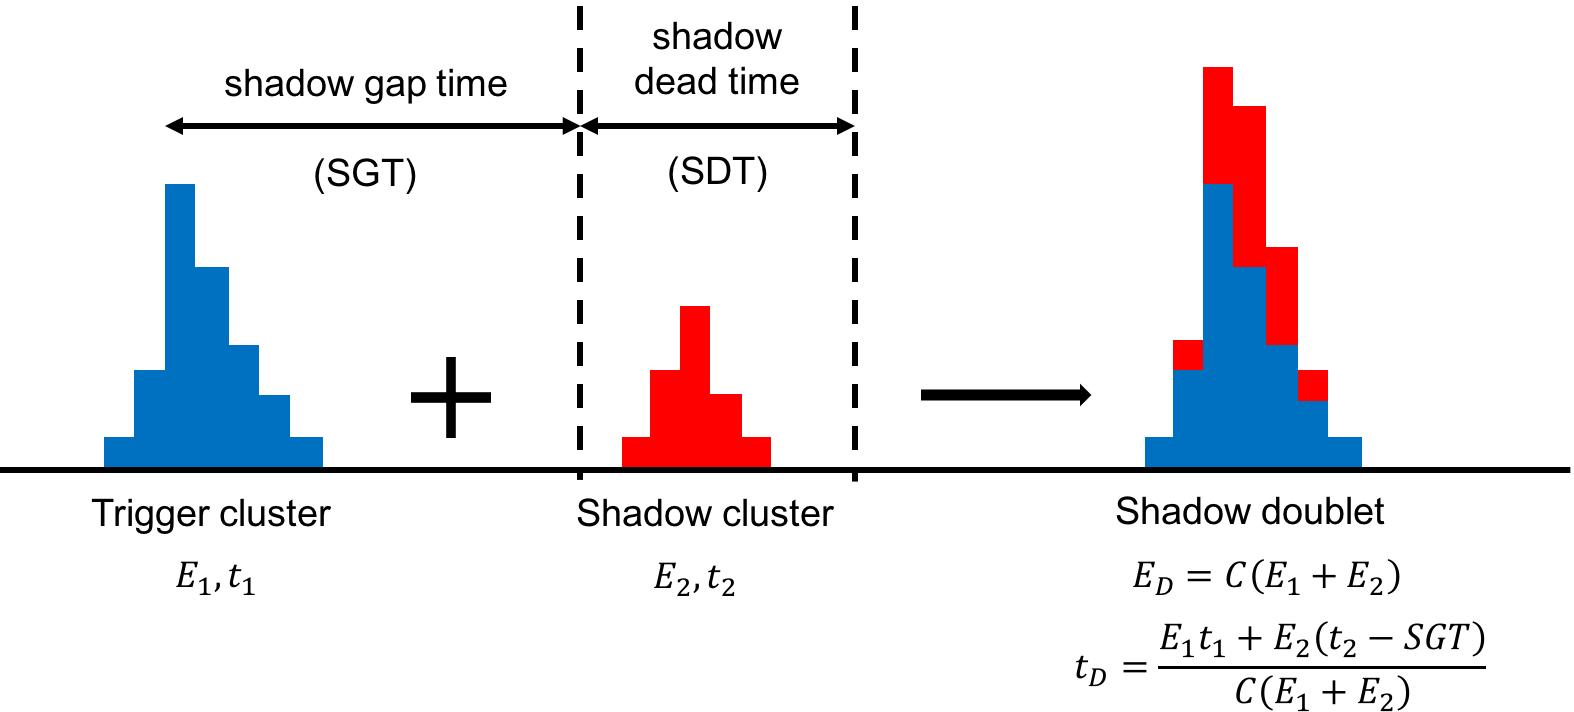
\includegraphics[width=\textwidth]{ShadowPileupMethod}
    \caption[Shadow pileup method]{The shadow pileup method looks for shadow clusters within a time window SDT, a small time away (SGT) from trigger clusters. If a shadow cluster is found, an artificial doublet is formed and included in the pileup spectra if it exceeds the chosen energy threshold.}
    \label{fig:ShadowPileupMethod}
\end{figure}


The pileup energy spectra as compared to the cluster energy spectra is shown in \figref{fig:ClusterEnergiesVsPileupEnergies}. In general, the two lobes starting at approximately $\SI{3}{\GeV}$ and $\SI{6}{\GeV}$ consist of double and triple pileup events respectively\footnote{All orders of pileup fill out the whole energy range, but certain areas consist of mostly one or the other.}. It can be seen that the shadow method of pileup construction produces a pileup energy spectra which is a decent approximation of the cluster energies above the maximum energy that a single decay positron would have at $(\SI{3.094}{\GeV}) + \text{detector resolution}$, for cases of double and even triple pileup. The shape difference arises from two factors: First, the shadow method is only written to construct doublets, and does not consider cases of triple or higher orders of pileup. Second, the real pileup in the data contaminates the construction of the shadow pileup spectra, such that a shadow doublet can be constructed from real pileup pulses. While this alleviates the triplet problem slightly, it means that the doublet pileup spectrum is slightly wrong. The corrected energy spectra (cluster energies minus pileup energies), can be seen in \figref{fig:AddedEnergies}. The shape mismatch is even more apparent as the corrected energy spectrum is high for energies above the expected tail of the true energy distribution, and then goes negative before tailing off to zero. 


    \begin{figure}[]
        \centering
        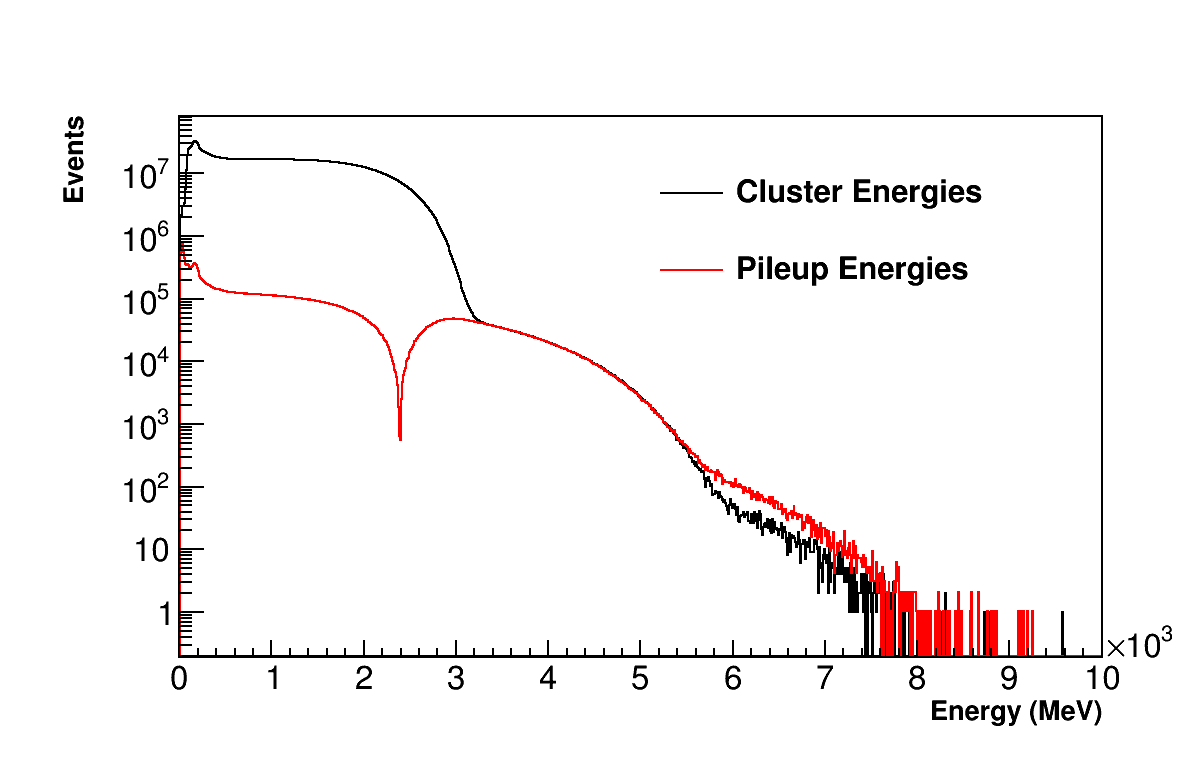
\includegraphics[width=\textwidth]{ClusterEnergiesVsPileupEnergies}
        \caption[Cluster energies vs pileup energies]{Cluster energies in black are plotted vs pileup energies in red, for all calorimeters added together, plotted on a log scale. At energies below about 2.4 GeV the pileup energy spectrum goes negative. In this plot the absolute value of the pileup energies is plotted, and a spike at about 2.4 GeV can be seen as a consequence of this. The shapes do not match perfectly for the constructed pileup spectra, which can be seen at high energies. It should be noted that for energies above $\SI{3.094}{\GeV}$ there is still a shape mis-match even though the red and black curves overlap due to the plotting scale. Data from the 60h dataset.}    
        \label{fig:ClusterEnergiesVsPileupEnergies}
    \end{figure}


    \begin{figure}[]
    \centering
        \begin{subfigure}[]{0.45\textwidth}
            \centering
            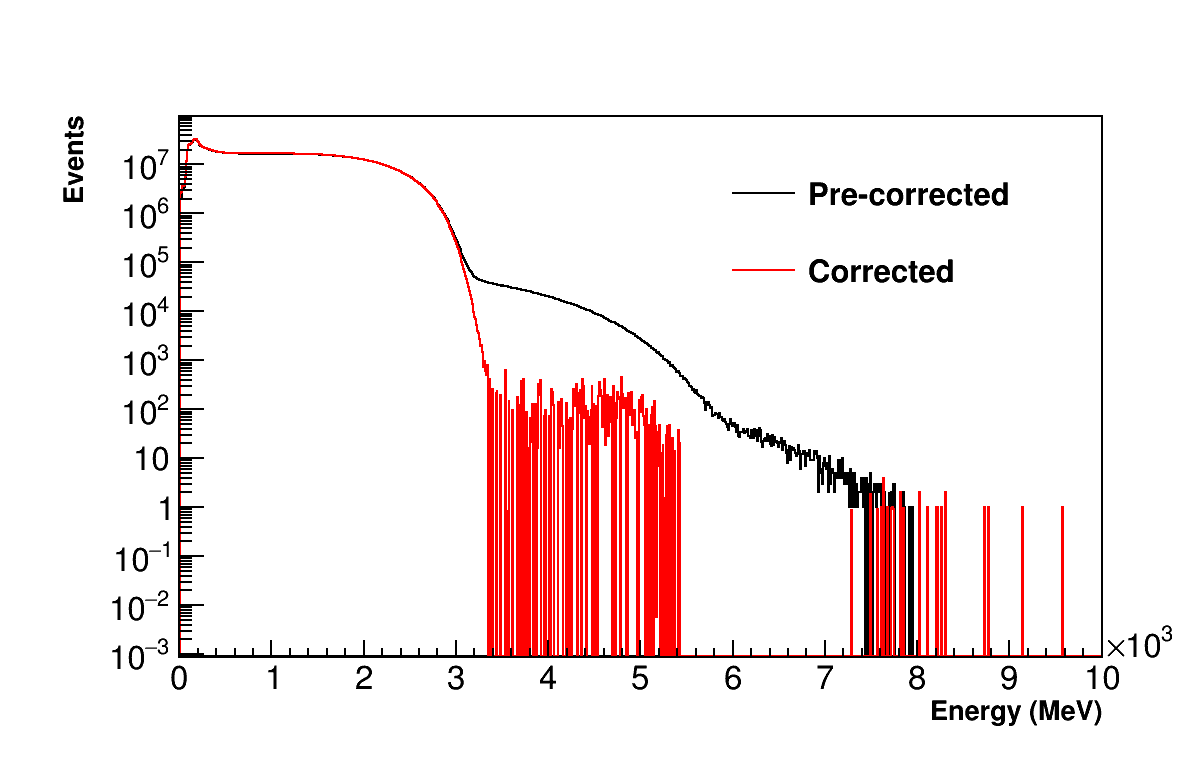
\includegraphics[width=\textwidth]{AddedEnergies}
            \caption{Log scale - the corrected energy spectrum goes negative around 5 GeV.}
        \end{subfigure}% %you need this % here to add spacing between subfigures
        \hspace{1cm}
        \begin{subfigure}[]{0.45\textwidth}
            \centering
            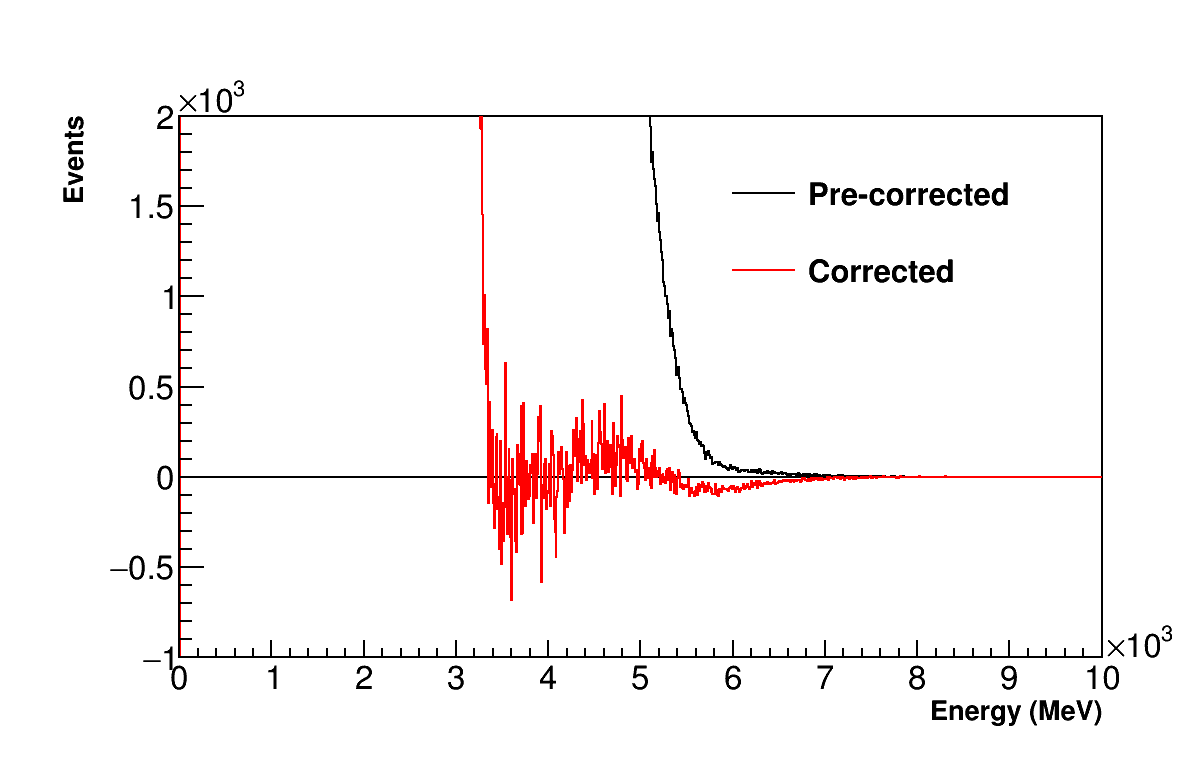
\includegraphics[width=\textwidth]{AddedEnergiesZoomed}
            \caption{Linear scale - zoomed in to show the shape.}
        \end{subfigure}
    \caption[Non-corrected and pileup corrected cluster energies]{Plots for the pre-corrected and corrected energy spectra are shown, all calorimeters added together. Because the triplets and contamination are not accounted for, the corrected energy spectrum does not lie exactly along zero above the energy response of the detectors. Data from the 60h dataset.}
    \label{fig:AddedEnergies}
    \end{figure}



In order to produce a slightly better estimate of the pileup, a multiplier can be applied to the pileup energy and time spectra. By taking the ratio of cluster energies over pileup energies and fitting the region where the energies are dominated by real pileup doublets, a correction factor of approximately 3\% is found, as shown in \figref{fig:EnergyRatio}. Similarly, the cluster times can be examined for cluster energies over \SI{3500}{\MeV}, where the clusters consist purely of pileup pulses, \figref{fig:PileupTimesRatio}. By taking the ratio of the pileup corrected times over all times, the level of residual pileup can be determined. Just as in the ratio of the energies, an approximately 3\% factor is found. When applying this multiplier, the cluster times above \SI{3.5}{\GeV} can be seen to be eliminated as in \figref{fig:PileupTimesRatio}. As will be shown in \secref{sub:pileuperror}, the scale of this multiplier is well within $1\sigma$ of the pileup multiplier error. The final pileup time spectrum for those pileup pulses above energy threshold is shown in \figref{fig:PileupTimeSpectrum}. 


    \begin{figure}[]
        \centering
        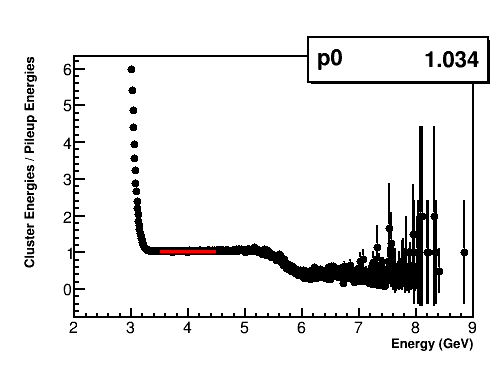
\includegraphics[width=.5\textwidth]{EnergyRatio}
        \caption[Cluster energies divided by pileup energies]{Cluster energies over pileup energies. A region from \SI{3500}{}--\SI{4500}{\MeV} is fit to a straight line, where the doublets dominate the energy distribution. Data from the 9d dataset.}    
        \label{fig:EnergyRatio}
    \end{figure}


    \begin{figure}[]
    \centering
        \begin{subfigure}[]{0.45\textwidth}
            \centering
            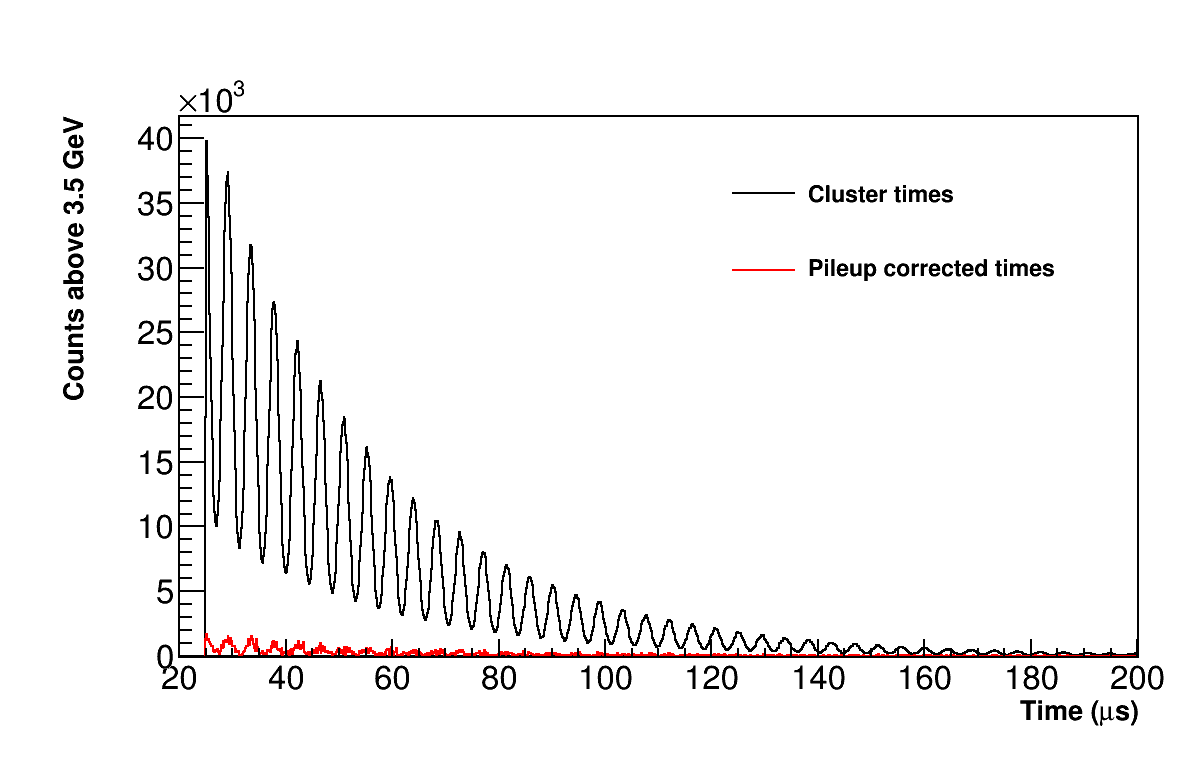
\includegraphics[width=\textwidth]{PileupSubtractedTimesComparison-NoAutoScaling}
            % \caption{Cluster t}
        \end{subfigure}% %you need this % here to add spacing between subfigures
        \hspace{1cm}
        \begin{subfigure}[]{0.45\textwidth}
            \centering
            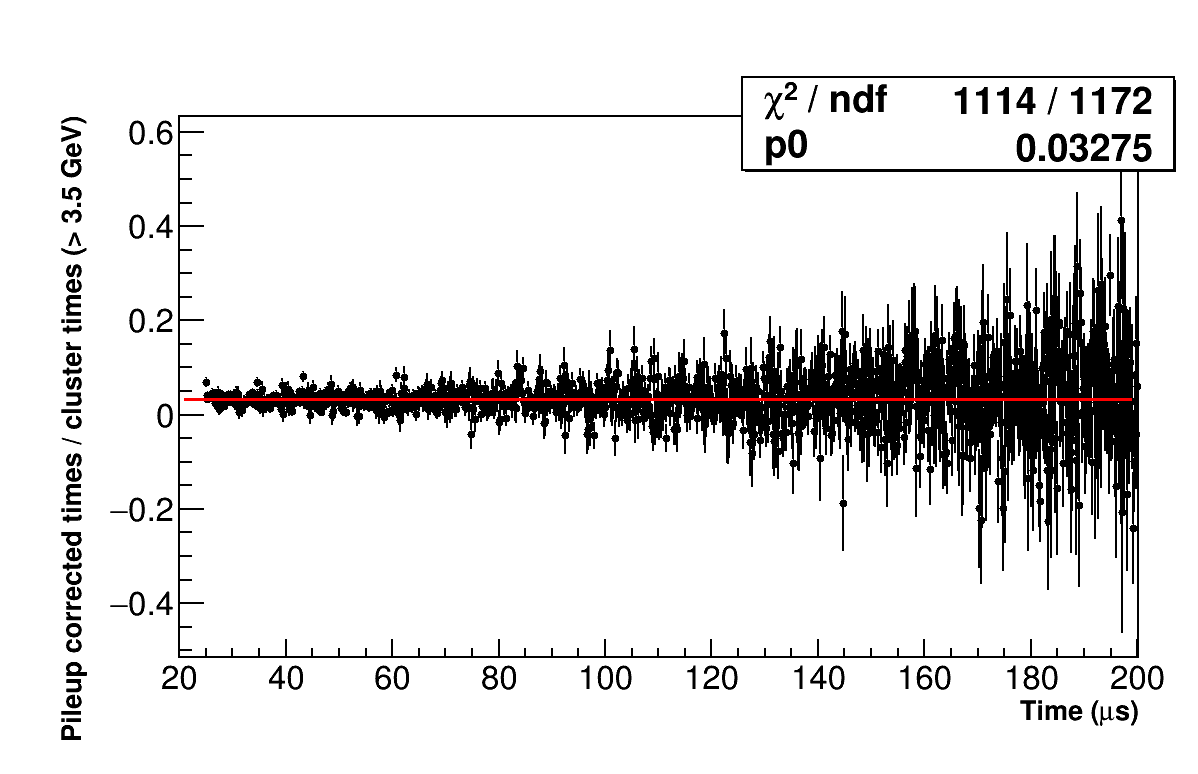
\includegraphics[width=\textwidth]{PileupSubtractedTimesRatio-NoAutoScaling}
            % \caption{}
        \end{subfigure}

        \begin{subfigure}[]{0.45\textwidth}
            \centering
            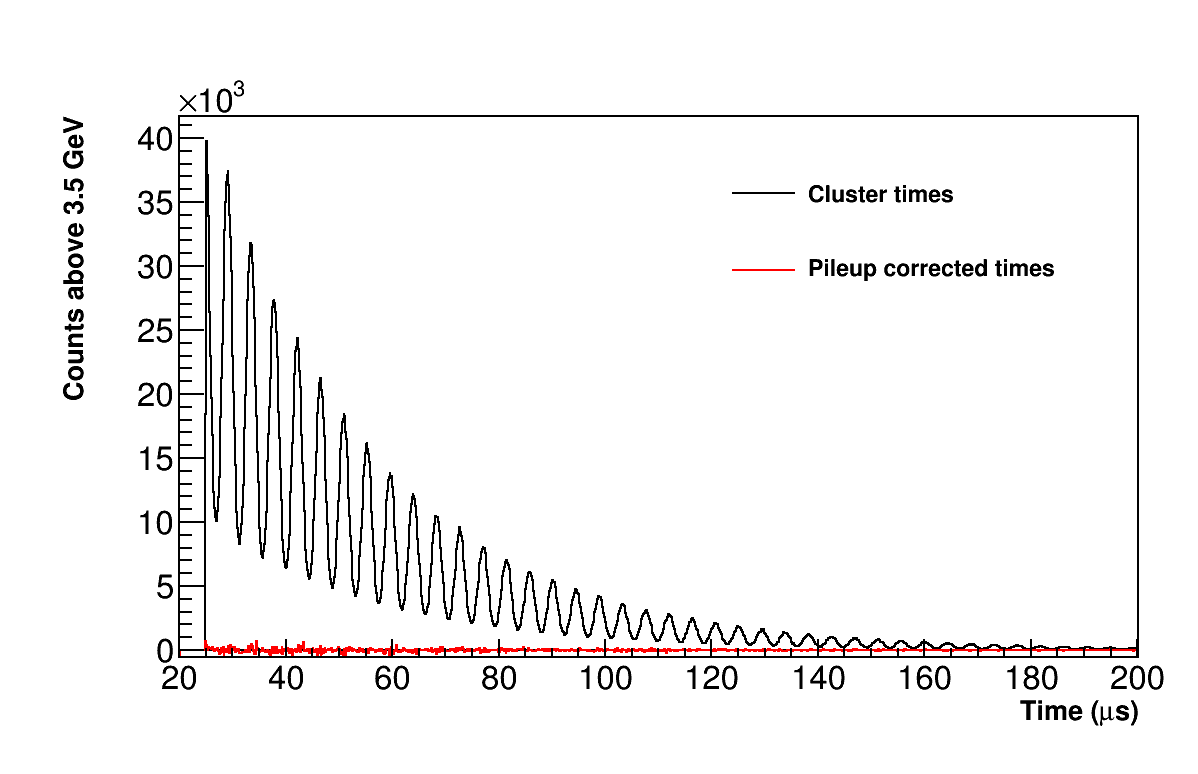
\includegraphics[width=\textwidth]{PileupSubtractedTimesComparison-AutoScaling}
            % \caption{}
        \end{subfigure}% %you need this % here to add spacing between subfigures
        \hspace{1cm}
        \begin{subfigure}[]{0.45\textwidth}
            \centering
            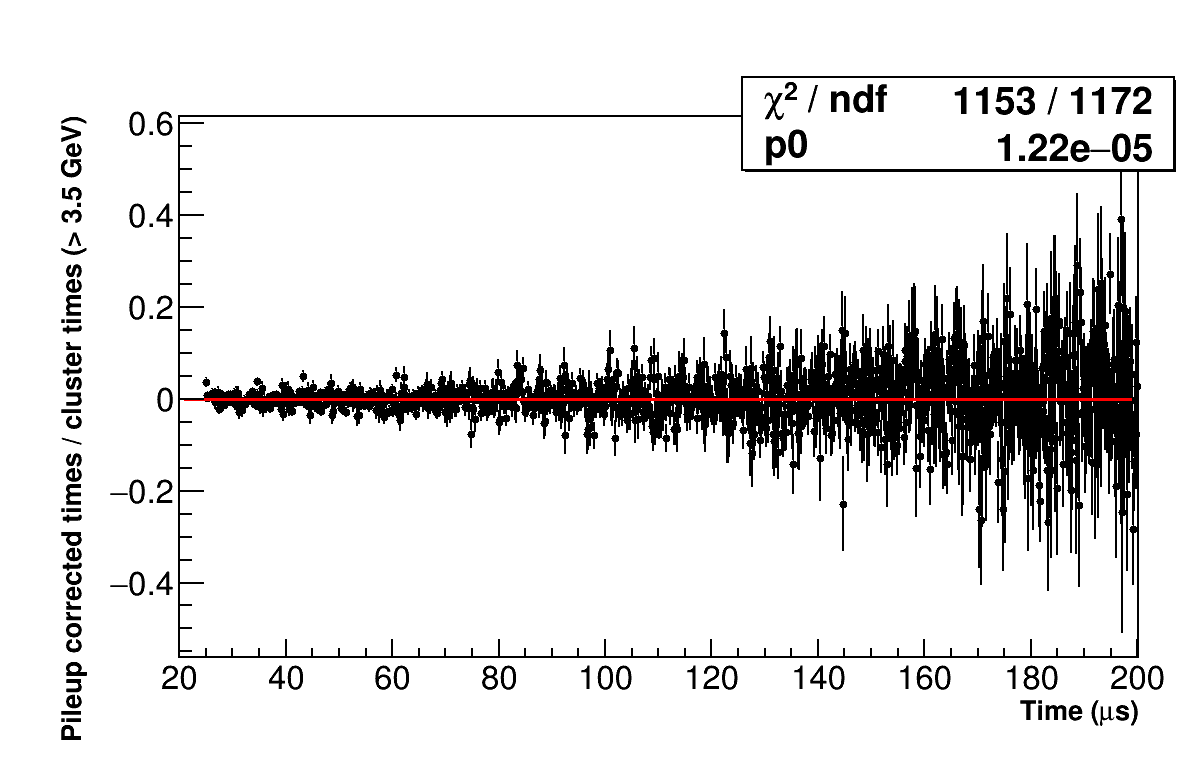
\includegraphics[width=\textwidth]{PileupSubtractedTimesRatio-AutoScaling}
            % \caption{}
        % \label{fig:correctedclustertimes}
        \end{subfigure}
    \caption[Cluster times above \SI{3.5}{\GeV}]{Cluster times and pileup corrected times for counts above \SI{3.5}{\GeV} (left) and their ratio (right). The top two plots are used to determine the approximate level of residual pileup left in the data, coming out to about 3\%. The bottom two plots show the application of that factor and the resulting removal of the remaining pileup. Data from the 9d dataset.}
    \label{fig:PileupTimesRatio}
    \end{figure}



    \begin{figure}[]
        \centering
        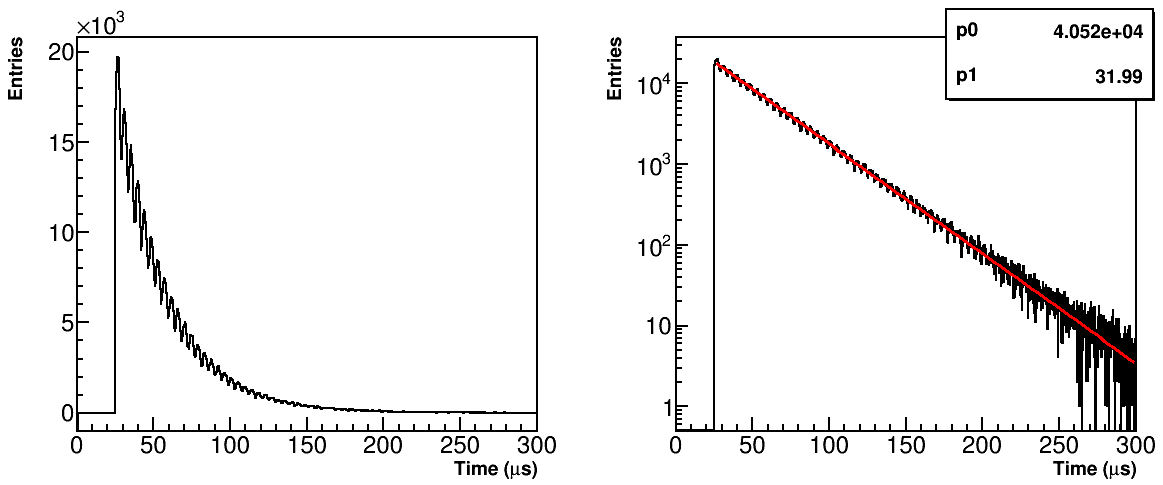
\includegraphics[width=\textwidth]{PileupTimeSpectrum}
        \caption[Pileup time spectrum above threshold]{Plotted is constructed pileup time spectrum on a linear (left) and log (right) scale. The histogram on the right is fit to a simple two parameter exponential to get an idea of the lifetime of the pileup, calculated here as $\SI{31.99}{\micro s}$, which is close to half of the muon lifetime at about $\SI{64.44}{\micro s}$. Data from the 60h dataset.}
        \label{fig:PileupTimeSpectrum}
    \end{figure}





It has been determined that regardless of any residual shape mismatch in the cluster times below \SI{3.5}{\GeV}, the systematic error on the extracted \wa frequency due to the pileup is within the target uncertainty for the level of statistics in the Run~1 dataset, \secref{sub:pileuperror}. For analyses past Run~1 where the error budget is reduced, it may be necessary to improve the shadow method to account for triplets and the contamination. Finally, since the pileup is statistically constructed and then subtracted from the data, the errors on the final time histogram are no longer Gaussian. The proper calculation of the errors is detailed in \appref{app:PileupErrors}.


% https://gm2-docdb.fnal.gov/cgi-bin/private/RetrieveFile?docid=13963&filename=PileupScaleShadowTesting.pdf&version=1
% https://gm2-docdb.fnal.gov/cgi-bin/private/RetrieveFile?docid=14394&filename=PileupFormEtc.pdf&version=2



\subsection{Ratio Method}
\label{sub:ratio_method}

% I put this here because technically the ratio method involves modifying the actual data that is being fit

The method used in this analysis to extract \wa is called the ``Ratio Method,'' or sometimes ``R-Method.'' It is a technique that modifies the data in such a way that the exponential decay in the time histogram is removed, and slow effects are reduced. It was used successfully in the E821 experiment \cite{JKThesis,LDThesis,JPThesis}. A full derivation of the equations in the method is given in \appref{app:RatioDerivation}; here is given a short summary. \figref{fig:RatioFormationFunctions} provides a pictorial representation of how the method works.

The method works by dividing the data into four separate datasets, one with the times of all clusters shifted up by half a \gmtwo period, $+$\Tatwo, one with cluster times shifted down by half a \gmtwo period, $-$\Tatwo, and two unchanged. Assuming the data is described by the five parameter function described in \secref{section:WaIntro} and shown in \figref{fig:fiveparamfunc}, %\equref{eq:5parfunc}
        \begin{align} \label{eq:5parfuncrepeated}
            N_{d}(t, E_{th}) = N_{0}(E_{th}) \cdot e^{-t/\gamma\tau_{\mu}} \cdot [1 + A(E_{th}) \cos(\omega_{a}t+\phi(E_{th}))],
        \end{align}
and that the data is equally split into four subsets, then the new four datasets are given as\footnote{When handling the pileup in the ratio method, the pileup time spectra are split into four datasets and time-shifted in the same way as the cluster hit times. Associated doublets and singlets are kept together in the same individual dataset, and the four pileup datasets are subtracted off their respective ratio datasets before forming the ratio.}:
    \begin{equation}
    \begin{aligned}
        u_{+}(t) &= \frac{1}{4} N_{5}(t+T/2) \\
        u_{-}(t) &= \frac{1}{4} N_{5}(t-T/2) \\
        v_{1}(t) &= \frac{1}{4} N_{5}(t) \\
        v_{2}(t) &= \frac{1}{4} N_{5}(t)
    \end{aligned}
    \end{equation}
In order to time shift the data as such, \Ta needs to be known a priori to high precision. The value used is taken from the E821 result, and its value is taken as $1/f_{a}$, where $f_{a}$ is \SI{0.2290735}{MHz}:
        \begin{align}
            T_{a} \approx \SI{4.365411}{\micro s}
        \label{eq:Ta}
        \end{align}
This value for $f_{a}$ was determined by averaging column 2 of Table XV of the E821 Final Report \cite{E821FinalReport}, which consits of the $f_{a}$ results for the different run periods in that experiment. A systematic error on the choice of this parameter is calculated in \secref{sub:TimeShiftingParameters}.


The datasets are then combined as 
    \begin{equation}
    \begin{aligned}
        U(t) &= u_{+}(t) + u_{-}(t), \\
        V(t) &= v_{1}(t) + v_{2}(t),
    \label{eq:UandV}
    \end{aligned}
    \end{equation}
both of which are shown in \figref{fig:UVfuncs}. It is immediately apparent that the $U(t)$ data are shifted 180\textdegree{} out of phase from the $V(t)$ data. The ratio is then defined as\footnote{The ratio can also be defined with $U(t) - V(t)$ in the numerator, however then the phase of the ratio spectrum is shifted 180\textdegree{} from the original $N_{5}(t)$ spectrum.}
    \begin{align}
        R(t) &= \frac{V(t) - U(t)}{V(t) + U(t)}
    \label{eq:ratioUV}
    \end{align}
where the numerator and denominator are plotted in Figures~\ref{fig:rationumfunc} and \ref{fig:ratiodenomfunc} respectively. The numerator is an exponentially decaying cosine, while the denominator is a simple exponential, both of which can be seen as originating from the difference and sum of the $U(t)$ and $V(t)$ data respectively. The resulting ratio spectrum can be seen in \figref{fig:ratiofunc}, where the exponential has been eliminated. The fit function is then reduced from five parameters down to three:
    \begin{align}
        R(t) \approx A \cos(\omega_{a}t) - C,
    \label{eq:ratiowithC}
    \end{align}
where  
    \begin{align}
        C = \frac{1}{16} \Big(\frac{T}{\tau}\Big)^{2} \approx 2.87 * 10^{-4},
    \end{align}
and these functions have been determined from the time-shifted five parameter function plugged into the $U(t)$ and $V(t)$ variables. In addition to the exponential being eliminated, any slow terms in the data get time-shifted and divided as well, such that the amplitude of said slow effects are reduced. For faster effects, the degree of cancellation of the effect is dependent on the frequency. Effects at frequencies which are an odd multiple of \wa are preserved while effects at an even multiple of \wa are completely cancelled out. An example is shown in \figref{fig:CancellationInRatioMethod}. While this makes fitting the data easier in some cases, in others it is a downside that effects which still need to be included in the fit function now have their amplitudes reduced, making them harder to fit.


    \begin{figure}[]
    \centering
        \begin{subfigure}[t]{0.45\textwidth}
            \centering
            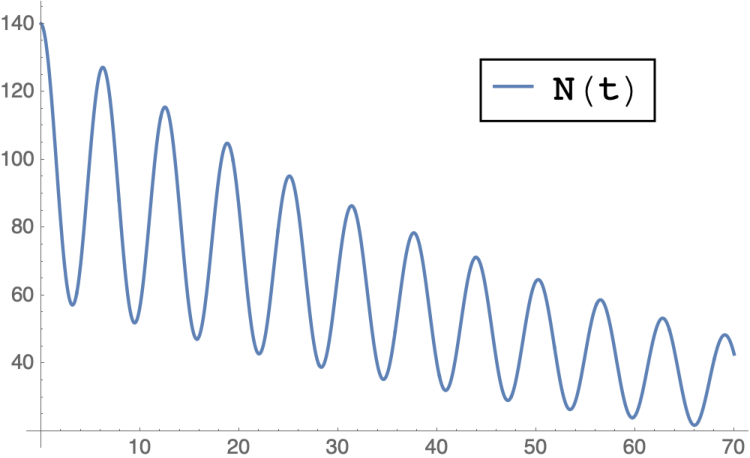
\includegraphics[width=\textwidth]{FiveParamFunc}
            \caption{The five parameter function defined in \equref{eq:5parfuncrepeated}, which describes the incoming data to first order.}
        \label{fig:fiveparamfunc}
        \end{subfigure}%

        \vspace{2mm}
        \begin{subfigure}[t]{0.45\textwidth}
            \centering
            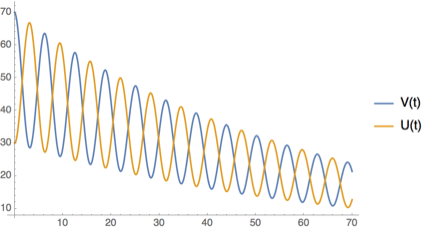
\includegraphics[width=\textwidth]{UVFuncs}
            \caption{$U(t)$ and $V(t)$ functions which describe the time-shifted and unshifted ratio datasets.}
        \label{fig:UVfuncs}
        \end{subfigure}
        \hspace{5mm}
        \begin{subfigure}[t]{0.45\textwidth}
            \centering
            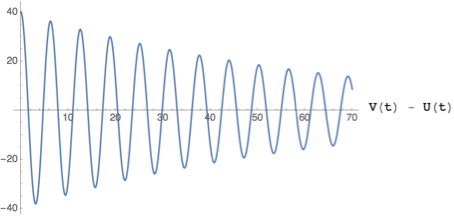
\includegraphics[width=\textwidth]{RatioNumFunc}
            \caption{The numerator function in the formed ratio, $V(t) - U(t)$. It is an exponentially decaying cosine.}
        \label{fig:rationumfunc}
        \end{subfigure}%
        \vspace{2mm}
        \begin{subfigure}[t]{0.45\textwidth}
            \centering
            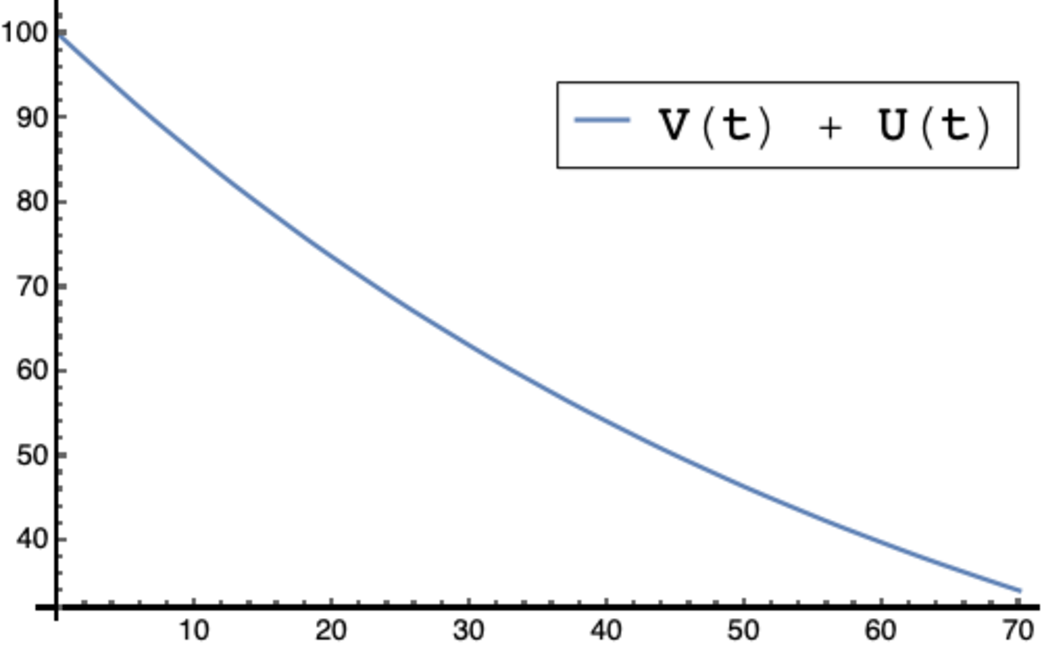
\includegraphics[width=\textwidth]{RatioDenomFunc}
            \caption{The denominator function in the formed ratio, $V(t) + U(t)$. It is an exponentially decaying curve.}
        \label{fig:ratiodenomfunc}
        \end{subfigure}
        \hspace{5mm}
        \begin{subfigure}[t]{0.45\textwidth}
            \centering
            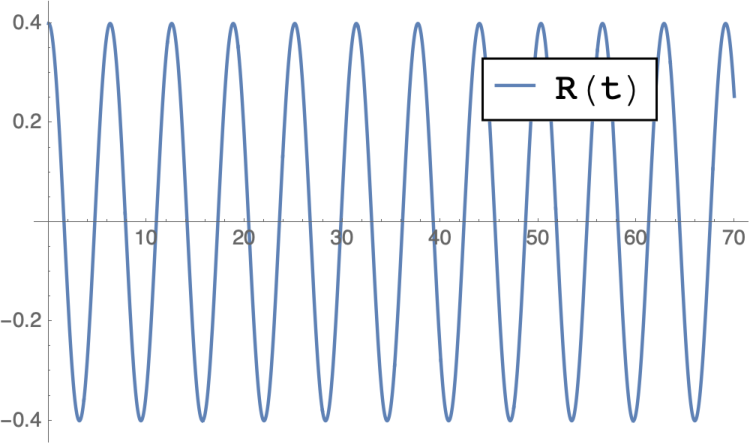
\includegraphics[width=\textwidth]{RatioFunc}
            \caption{The formed ratio function, describing the data after it has been handled as described in the text. To first order it is reduced to a simple cosine form.}
        \label{fig:ratiofunc}
        \end{subfigure}% 
    \caption[Ratio formation functions]{Functions describing the formation of the ratio in the data.}
    \label{fig:RatioFormationFunctions}
    \end{figure}


    \begin{figure}[]
        \centering
        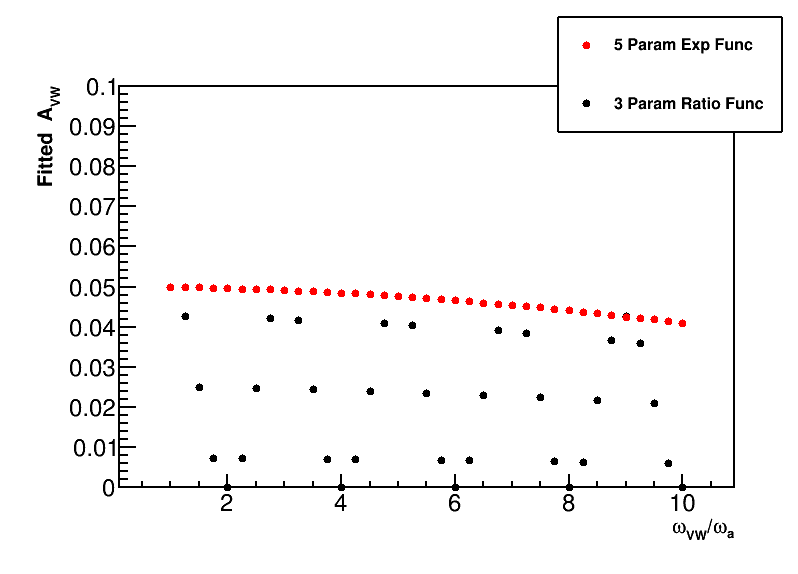
\includegraphics[width=.6\textwidth]{Fitted_Avw_Vs_Wvw_1x-10x}
        \caption[Cancellation of effect in Ratio Method versus frequency]{Fitted amplitude for a VW effect as a function of frequency in units of \wa in a Toy MC simulation, with a five parameter function in red and a three parameter ratio function in black. The input amplitude was 0.05. The fall off of red points is due to the high frequencies relative to the bin widths leading to an underestimate of the amplitude; performing an integral fit removes this trend. As shown the amplitude of the effect goes to zero for frequencies which are an even multiple of \wa.}
        \label{fig:CancellationInRatioMethod}
    \end{figure}



 In order to eliminate the constant $C$ at the end of \equref{eq:ratiowithC}, a different weighting scheme can be used as described in \refref{statisticspaper}:
    \begin{equation}
    \begin{aligned}
        u_{+}(t) &= \frac{e^{T/2\tau}}{2 + e^{T/2\tau} + e^{-T/2\tau}} N_{5}(t+T/2) \\
        u_{-}(t) &= \frac{e^{-T/2\tau}}{2 + e^{T/2\tau} + e^{-T/2\tau}} N_{5}(t-T/2) \\
        v_{1}(t) &= \frac{1}{2 + e^{T/2\tau} + e^{-T/2\tau}} N_{5}(t) \\
        v_{2}(t) &= \frac{1}{2 + e^{T/2\tau} + e^{-T/2\tau}} N_{5}(t)
    \label{eqn:fourHistsInText}
    \end{aligned}
    \end{equation}
Here $\tau = \gamma\tau_{\mu}$, and the factors out front are each close to $1/4$ and account for the degree of muon decay over a time period of \Tatwo. Similar to \Ta, the muon lifetime must be known a priori. It's value is taken as \mus{64.44}, determined from fits to the data. A systematic study regarding this parameter is described in \secref{sub:TimeShiftingParameters}. The ratio spectrum is then almost exactly described by just the cosine term,
    \begin{align} \label{eq:threeparamratio}
        R(t) \approx A \cos(\omega_{a}t),
    \end{align}
in the absence of other effects in the data. 




\section{Fitting the data}
\label{sec:Fitting}


The basic five parameter function used to the fit the data as described before is given as\footnote{In all cases here and onwards the actual fit parameters are in bold.}
    \begin{align}
        f(t) = \boldsymbol{N_{0}} \cdot e^{-t/\boldsymbol{\tau}} \cdot (1 + \boldsymbol{A} \cdot \cos(\omega_{a}t + \boldsymbol{\phi})),
    \label{eq:fiveparfuncagain}
    \end{align}
where the fit parameter for \wa is recast in terms of a ppm level shift \textbf{R} on a reference frequency,
    \begin{align}
        \omega_{a} = 2 \pi \cdot \SI{0.2291}{MHz} \cdot (1 + \textbf{R} \times 10^{-6}).
    \label{eq:wablind}
    \end{align}
This reference frequency of $\SI{0.2291}{MHz}$ was the same reference frequency used in E821, and \textbf{R} is blinded at the hardware and software levels \cite{ClockManual,SoftwareBlinding}. Fitting the data with \equref{eq:fiveparfuncagain} however is insufficient to properly describe the data. \figref{fig:FFT_fiveParameter} shows there are peaks in the FFT due to beam dynamics frequencies corresponding to the CBO, VW, and some beat frequencies with \wa. In order to properly account for these effects, additional terms need to be added to the fit function. 

    \begin{figure}[]
        \centering
        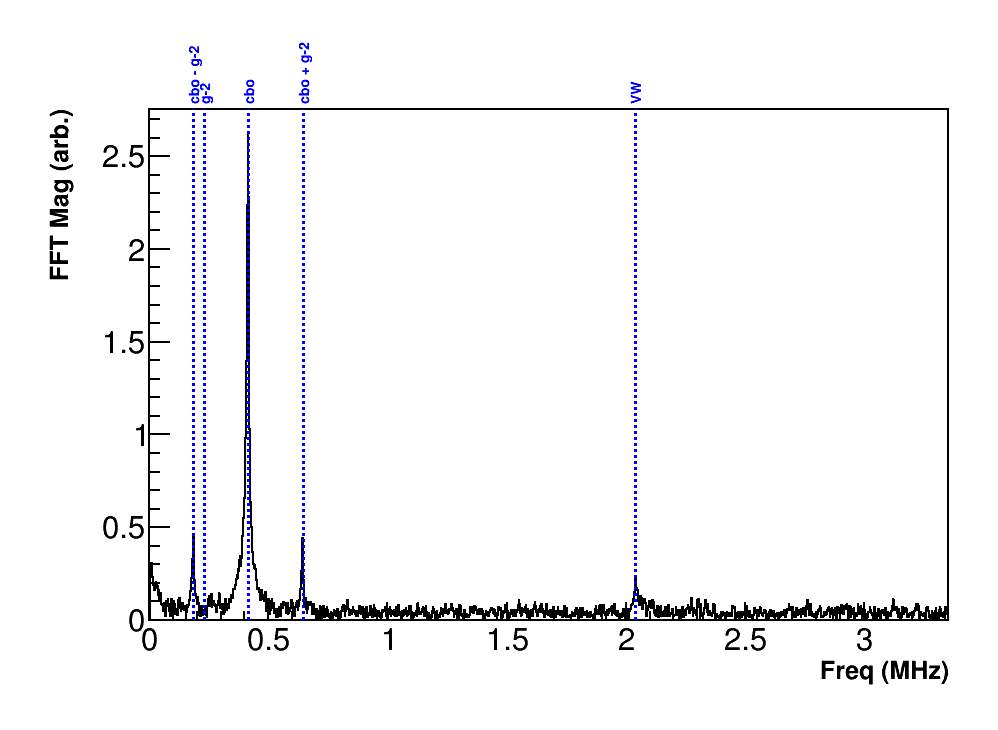
\includegraphics[width=.8\textwidth]{FFT_fiveParameter}
        \caption[FFT of five parameter fit residuals]{FFT of five parameter fit residuals. Peaks corresponding to beam dynamics frequencies of the CBO and VW and some beat frequencies with \wa are readily apparent. A rise at low frequencies corresponds to the effects of the lost muons in the data. From the 60h dataset.}
        \label{fig:FFT_fiveParameter}
    \end{figure}

\equref{eq:fiveparfuncagain} can be expanded to 
    \begin{align}
        f(t) = \Lambda(t) \cdot V(t) \cdot N_{cbo}(t) \cdot \boldsymbol{N_{0}} \cdot e^{-t/\boldsymbol{\tau}} \cdot (1 + A_{cbo}(t) \cdot \cos(\omega_{a}t + \phi_{cbo}(t))),
    \label{eq:TmethodFunction}
    \end{align}
where many additional terms have been added in order to account for effects in the data. The various additional terms $\{N_{cbo}(t), A_{cbo}(t), \phi_{cbo}(t), V(t), \Lambda(t)\}$ are described in the following sections. Fitting the data with this function, referred to as the ``Threshold Method'' or just ``T-Method,'' while not the subject of this dissertation, was done in this analysis as a diagnostic and informative tool for the Ratio Method analysis. 


In order to fit the ratio time spectra as constucted in \secref{sub:ratio_method}, a different function is used. While the immediate inclination is to use an expansion of \equref{eq:threeparamratio} with included additional effects similar to the T-Method fit function, instead the fit function used is a return to the explicit definition of the construction of the ratio time spectra in Equations~\ref{eq:UandV} and \ref{eq:ratioUV}. Including the additional effects previously mentioned, the fit function goes as
    \begin{gather}
        R(t) = \frac{2f(t) - f_{+}(t) - f_{-}(t)}{2f(t) + f_{+}(t) + f_{-}(t)}, \\
        f_{\pm}(t) = f(t \pm T_{a}/2), \\
        f(t) = \Lambda(t) \cdot V(t) \cdot N_{cbo}(t) \cdot (1 + A_{cbo}(t) \cdot \cos(\omega_{a}t + \phi_{cbo}(t))).
    \label{eq:fullratiofunction}
    \end{gather}
The $f(t)$ given here differs from that in \equref{eq:TmethodFunction} in that the $\boldsymbol{N_{0}} \cdot e^{-t/\boldsymbol{\tau}}$ terms have divided out, thus reducing the number of fit parameters necessary to model the data. Using this function as opposed to an expansion of the three parameter ratio function eliminates any approximations made in that three parameter function derivation, and any fit parameters should be consistent in value between the T-Method and Ratio Method results, barring adjustments due to the application of the Ratio Method. It should be noted here that while the Ratio Method reduces the sensitivity of the \wa extraction to various effects in the data, those effects typically still need to be included in the fit function for a proper estimatation of \wa. Because of the reduction in sensitivity, there are some parameters which the ratio has trouble fitting by itself. Using the T-Method fit function is then a useful tool for constraining these specific parameters.



\subsection{CBO terms}
\label{sub:cboterms}


As described in \secref{sub:CBO}, the CBO modulates the \wa oscillation. This shows up as a modification on the five parameter function parameters $\{N_{0}, A, \phi\} \rightarrow \{N_{0} \cdot N_{cbo}(t), A_{cbo}(t), \phi_{cbo}(t)\}$ where these terms are given to first order as
    \begin{align}
        N_{cbo}(t) &= (1 + \boldsymbol{A_{cbo-N}} \cdot e^{-t/\boldsymbol{\tau_{cbo}}} \cdot \cos(\omega_{cbo}(t) \cdot t + \boldsymbol{\phi_{cbo-N}})) \label{eq:Ncbo} \\ 
        A_{cbo}(t) &= \boldsymbol{A} \cdot (1 + \boldsymbol{A_{cbo-A}} \cdot e^{-t/\boldsymbol{\tau_{cbo}}} \cdot \cos(\omega_{cbo}(t) \cdot t + \boldsymbol{\phi_{cbo-A}})) \label{eq:Acbo} \\ 
        \phi_{cbo}(t) &= \boldsymbol{\phi_{0}} + \boldsymbol{A_{cbo-\phi}} \cdot e^{-t/\boldsymbol{\tau_{cbo}}} \cdot \cos(\omega_{cbo}(t) \cdot t + \boldsymbol{\phi_{cbo-\phi}}) \label{eq:Phicbo}
    \end{align}
In \equref{eq:Ncbo} the $N_{0}$ term is left out since the ratio fit includes the $N_{cbo}(t)$ term but not $N_{0}$, and in \equref{eq:Phicbo}, $\phi_{cbo}(t)$ has an additive phase instead of a multiplicative one since $\phi_{0}$ is not an amplitude and can be equal to zero. Each of the terms then includes additional fit parameters in an extra amplitude and phase, as well as one shared CBO lifetime and frequency. As described in \secref{sec:MuonBeamMeasurements}, the default model for the CBO modulation is assumed as an exponenetially decaying envelope. The CBO frequency, $\omega_{cbo}(t)$, was time-dependent for Run~1 as found in \secref{sec:MuonBeamMeasurements}. The function for the CBO frequency shown in \figref{fig:CBOFrequency} is given in the fit function as
    \begin{align} \label{eq:CBOfreqForm}
        \omega_{cbo}(t) = \boldsymbol{\omega_{cbo}} \cdot \Big(1 + \frac{Ae^{(-t/\tau_{A})}}{\omega_{0}t} + \frac{Be^{(-t/\tau_{B})}}{\omega_{0}t}\Big),
    \end{align}
where $\boldsymbol{\omega_{cbo}}$ is the free fit parameter, and the model parameters $\{\omega_{0}, A, \tau_{A}, B, \tau_{B}\}$ are fixed from the tracking analysis. These parameters for the various datasets and two tracker stations are given in \tabref{tab:CBOFrequencyParameters}. 



% \begin{landscape}
\begin{table}[]
\centering
\small
\setlength\tabcolsep{10pt}
\renewcommand{\arraystretch}{1.2}
\begin{tabular*}{1\linewidth}{@{\extracolsep{\fill}}lcccccc}
  \hline
    \multicolumn{7}{c}{\textbf{CBO Frequency Model Parameters}} \\
  \hline\hline
    Dataset & Tracker Station & $\omega_{0}$ (rad/\mus{}) & $A$ (rad) & $\tau_{A}$ (\mus{}) & $B$ (rad) & $\tau_{B}$ (\mus{}) \\
  \hline
    \multirow{2}{*}{60h} & 12 & 2.3389 & 2.9 & 81.8 & 5.12 & 7.7 \\
                         & 18 & 2.3387 & 2.82 & 81.1 & 5.08 & 8.2 \\
  \hline
    \multirow{2}{*}{HighKick} & 12 & 2.6145 & 3.27 & 52.8 & 6.96 & 6.6 \\
                              & 18 & 2.6137 & 3.23 & 46.2 & 6.61 & 6.8 \\
  \hline
    \multirow{2}{*}{9d} & 12 & 2.6106 & 2.86 & 72.8 & 5.50 & 8.5 \\
                        & 18 & 2.6110 & 2.89 & 79.2 & 5.44 & 9.2 \\
  % \hline
  %   \multirow{2}{*}{LowKick} & 12 &  &  &  &  &  \\
  %                            & 18 &  &  &  &  &  \\
  % \hline
  %   \multirow{2}{.07\textwidth}{SuperLowKick} & 12 &  &  &  &  &  \\
  %                                             & 18 &  &  &  &  &  \\
  \hline
    \multirow{2}{*}{Endgame} & 12 & 2.3377 & 7.43 & 95.1 & 4.71 & 9.0 \\
                             & 18 & 2.3379 & 7.44 & 95.2 & 4.90 & 9.2 \\                                                        
  \hline
\end{tabular*}
\caption[Dataset CBO frequency model parameters]{Fixed parameters in the CBO frequency model \cite{CBOFreqTrackingElog,JamesPersonalComm}. \textbf{Here I source personal communication with James, as I don't think there's a source for the HighKick numbers.}}
\label{tab:CBOFrequencyParameters}
\end{table}
% \end{landscape}


It should be noted that Equations~\ref{eq:Acbo} and \ref{eq:Phicbo} are not necessarily needed in order to get good fits to the data (whereas \equref{eq:Ncbo} always is). This is typically dataset or random seed dependent. While some datasets had certain parameters with large errors relative to their amplitudes, for this analysis all terms were successfully included in all dataset fits with appropriate tuning of the starting parameters with well converging fits. 


When considering higher order CBO modifications to the fit function, the only term that was found to be fittable was the second order CBO modulation on the $\boldsymbol{N_{0}}$ term, 
    \begin{align}
        N_{2cbo}(t) &= (1 + \boldsymbol{A_{2cbo-N}} \cdot e^{-2t/\boldsymbol{\tau_{cbo}}} \cdot \cos(\omega_{cbo}(t) \cdot t + \boldsymbol{\phi_{2cbo-N}})). \label{eq:N2cbo}
    \end{align}
This stands to reason as the $N_{cbo}(t)$ is the largest CBO effect. The form is assumed to be the same as the first order CBO terms, except the lifetime of the effect is half the CBO lifetime, $\tau_{cbo}/2$. This is due to the fact that the $N_{2cbo}(t)$ is reasoned to come from the width of the oscillating beam, as opposed to the oscillating mean. Indeed as will be shown in \secref{sub:per_calorimeter_fits}, the inclusion of this term is necessary to get good fits to the per calorimeter data, where the CBO effect is stronger compared to in the sum of the calorimeter data. For this reason, and again because the $N_{2cbo}(t)$ term is fittable in the calorimeter sum data, this term is included in fits to each of the datasets.


Systematic studies relating to the choice of envelope and choice of fixed parameters in the frequency model are explored in \secref{sub:cboerror}. For future runs beyond Run~1, it may be necessary to include the higher order modifications to the $\boldsymbol{A}$ and $\boldsymbol{\phi}$ terms.



\subsection{VW term}
\label{sub:vw_term}

As mentioned briefly at the end of \secref{sec:Histogramming}, the VW effect is time-randomized out of the data, such that $V(t) = 1$. This is done due to complications with the Ratio Method. In the 60h and Endgame datasets, the VW frequency was found to be nearly 10 $\cdot$ \wa, on a potential resonance. While to first order this even multiple frequency implies the VW effect should completely cancel out in the Ratio Method, \figref{fig:CancellationInRatioMethod}, the FR effect in combination with the VW leads to a modified envelope for the VW effect in the Ratio Method fits and inflated VW amplitudes \cite{VWinRatio}. See Figures~\ref{fig:VWresonance} and \ref{fig:JamesMC_VW_FR}.

\begin{figure}[]
    \centering
    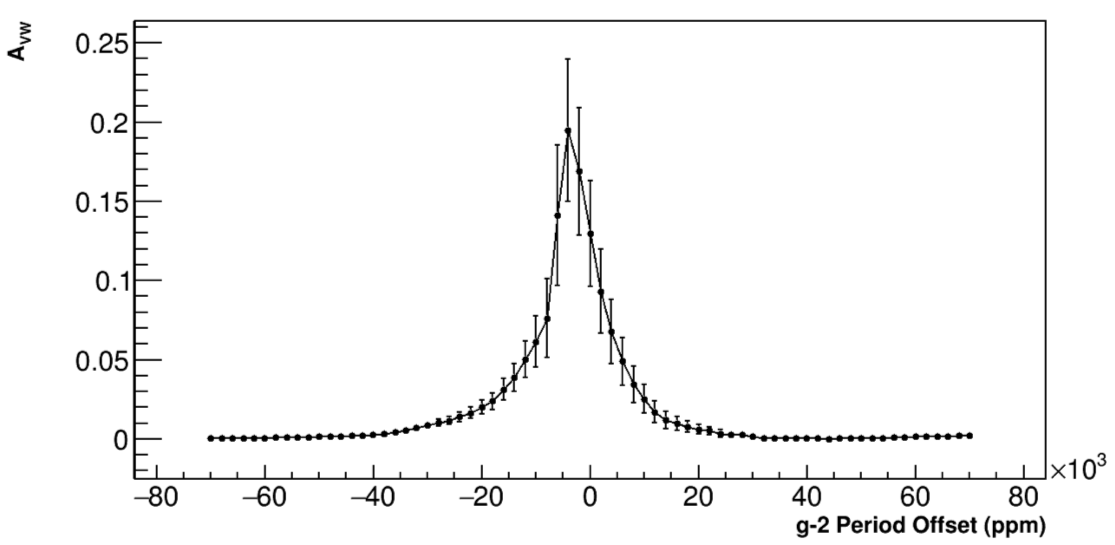
\includegraphics[width=.7\textwidth]{AvwResonance_60h}
    \caption[VW amplitude resonance in the 60h dataset]{Fitted VW amplitude as a function of the choice of  offset from $T_{a}$ in units of thousands of ppm for the 60h dataset. The default time-shift lies at 0 on this plot, right on the resonance where the VW amplitude blows up. Only by time-shifting by a drastically different amount (which negatively affects R), can the resonance be avoided.}
    \label{fig:VWresonance}
\end{figure}


\begin{figure}[]
\centering
    \begin{subfigure}[t]{0.6\textwidth}
        \centering
        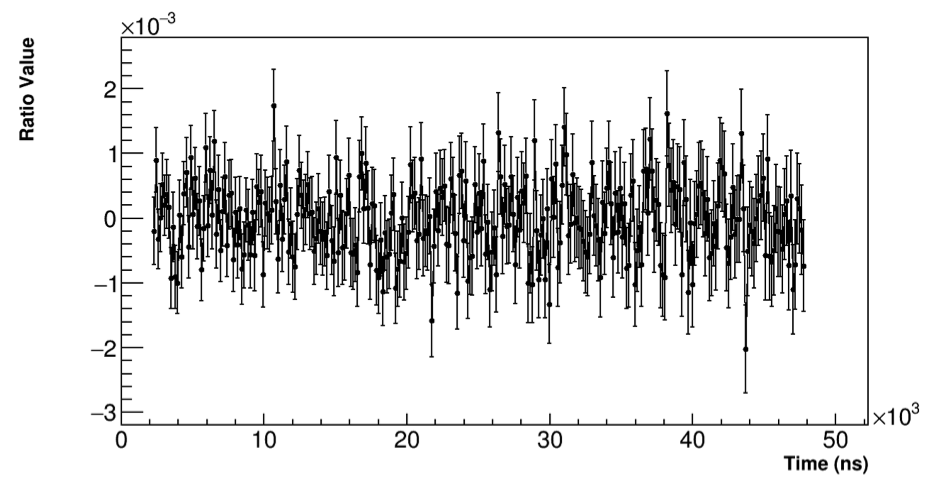
\includegraphics[width=\textwidth]{JamesMC_noFR}
        \caption{Without the FR effect included.}
    \end{subfigure}%

    \begin{subfigure}[t]{0.6\textwidth}
        \centering
        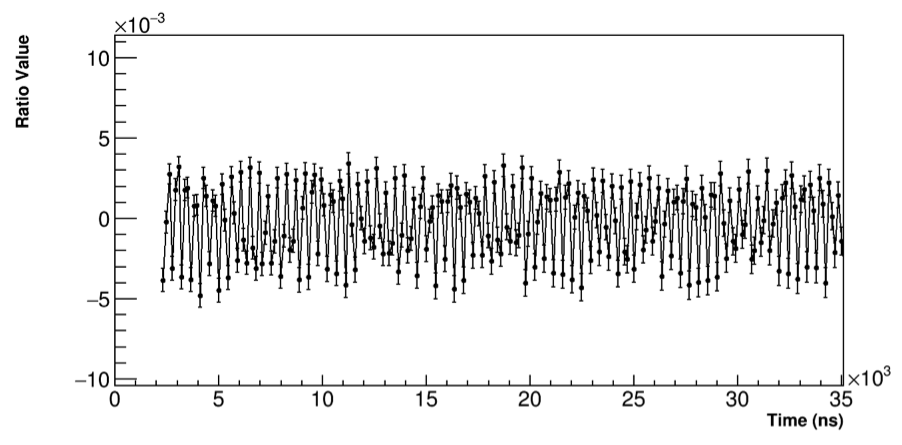
\includegraphics[width=\textwidth]{JamesMC_withFR}
        \caption{With the FR effect included.}
    \end{subfigure}
\caption[]{Ratio data with and without the FR effect from a Toy MC simulation, with a VW effect with a frequency $\omega_{VW} = 10 \cdot \omega_{a}$. The \wa wiggle itself has been removed, and the lifetime of the VW was set to a large number. The top plot shows ratio data which is consistent with 0 after all effects have been removed and the VW has divided out. The bottom plot shows ratio data inconsistent with 0, with oscillations at the VW frequency, and an interesting beating structure. Note the different scales.}
\label{fig:JamesMC_VW_FR}
\end{figure}


For the 9d dataset which has a VW frequency that's nearly 9 $\cdot$ \wa and avoids said resonance (and by extension the HighKick), it was found that the Ratio Method flattened out the VW amplitudes as a function of calorimeter number leading to a systematically smaller VW amplitude in the calorimeter sum fit. The simplest solution to remove both of these problems was to randomize out the VW effect entirely. \tabref{tab:A_change} gives the change in asymmetry and corresponding change in the statistical error on R due to this added time randomization for three of the Run~1 datasets. It was found that the added randomization increased the statistical error on R by a negligible amount for the Run~1 analysis. It was also found that the added level of time-randomization changed the mean value of R for many random seed fits to the data by a small amount, statistically consistent without the extra randomization \cite{VWinRatio}. Going forward for the future runs, it may be necessary to include the proper VW envelope in the fits using a functional form of the FR instead of randomizing out the effect.

\begin{table}[]
\centering
\small
\setlength\tabcolsep{10pt}
\renewcommand{\arraystretch}{1.2}
\begin{tabular*}{1\linewidth}{@{\extracolsep{\fill}}lcccc}
  \hline
    \multicolumn{5}{c}{\textbf{Change in Asymmetry due to VW Randomization}} \\
  \hline\hline
    Dataset & $A$ no randomization & $A$ with randomization & $\Delta A$ & $\Delta \sigma_{R}$ (ppb) \\
  \hline
    60h & $0.3697$ & $0.3637$ & $-0.0060$ & $22.7$ \\
  \hline
    9d & $0.3714$ & $0.3639$ & $-0.0075$ & $18.1$ \\
  \hline
    Endgame & $0.3747$ & $0.3686$ & $-0.0061$ & $10.7$ \\
  \hline
\end{tabular*}
\caption[]{Asymmetry values in three of the Run~1 datasets with and without the VW randomization, and the corresponding change in the statistical error on R. An energy cut of 1700 MeV was applied to the data. The HighKick dataset has the lowest asymmetry and the least statistics, so the increase in the statistical error would be negligible as it is for the other datasets.}
\label{tab:A_change}
\end{table}



Barring the envelope changes in the Ratio Method, here is still given the form for the VW as it is used in the T-Method fits. The form for the VW term is taken identically to the CBO terms, 
    \begin{align} \label{eq:VWterm}
        V(t) = 1 + \boldsymbol{A_{VW}} \cdot e^{-t/\boldsymbol{\tau_{VW}}} \cos(\omega_{VW}(t) \cdot t + \boldsymbol{\phi_{VW}}), 
    \end{align}
with an exponentially decaying envelope, and an additional amplitude and phase parameter. The VW frequency $\omega_{VW}$ is given in \equref{eq:VWfreq}, where it is seen to be dependent on the cyclotron frequency and vertical betatron frequency. Using Equations~\ref{eq:tunes} and \ref{eq:CBOfreq}, the dependence on the CBO frequency is seen as
    \begin{equation}
    \begin{aligned}
        \omega_{VW}(t) &= 2\pi (f_{c} - 2f_{y_{BO}}), \\
                    % &= 2\pi \Big[f_{c} - 2f_{cbo}\sqrt{\frac{2f_{c}}{f_{cbo}}-1}\Big]
                    &= 2\pi \Big(f_{c} - 2f_{cbo}(t)\sqrt{2f_{c}/f_{cbo}(t)-1}\Big),
    \label{eq:VWfreqOne}
    \end{aligned}
    \end{equation}
where $f_{cbo}(t) = \omega_{cbo}(t)/2\pi$ is determined in the tracking analysis as described in \secref{sub:cboterms} and given by \equref{eq:CBOfreqForm}. While \equref{eq:VWfreqOne} is the theoretical frequency for the VW effect, it was found in the tracking analysis that including an adjustment factor on the CBO frequency $f_{cbo} \rightarrow \kappa f_{cbo}$ on the order of about a percent resulted in better agreement with the directly measured VW frequency \cite{cbofrequency,verticalbetatron}. In the fitting function itself, the VW frequency is then taken as
    \begin{align} \label{eq:VWfreqKappa}
        \omega_{VW}(t) = 2\pi \Big(f_{c} - 2 \cdot \boldsymbol{\kappa_{VW}} \cdot f_{cbo}(t)\sqrt{2f_{c}/(\boldsymbol{\kappa_{VW}} \cdot f_{cbo}(t))-1}\Big),
    \end{align}
where now the VW frequency fit parameter is $\boldsymbol{\kappa_{VW}}$. The origin of this extra factor is unclear, whether it is a tracker measurement issue, something to do with the frequency function approximation, or if it has something to do with the electrostatic quadrupoles. The inclusion of the extra factor however provides better fits and so it is kept in.




\subsection{Lost muons}
\label{subsec:lostmuons}


Muons lost from the storage ring during the frequency analyis portion of each fill will distort the observed decay positron spectrum. These muon losses typically originate from those muons with larger betatron amplitudes impacting material near the edge of the storage ring, thus losing energy and spiralling inward out of the ring, or from those muons which experience local field inhomogeneities and have their trajectories modified. A fraction of these lost muons will then pass through multiple calorimeters. Because lost muons are minimum-ionizing particles (MIPs), they will deposit a small amount of energy in hit calorimeters, around 170 \MeV as shown in \figref{fig:energyHist}. These lost muons typically have a flight time between adjacent calorimeters of \ns{6.5} \cite{lostmuonspaper,lostmuonsDenverTalk}. The $\Delta t$ and energy deposition distributions are shown in \figref{fig:lostmuondistributions}. By looking for coincidences between three adjacent calorimeters and then subtracting backgrounds, a pure sample of lost muons can be constructed. The lost muon spectrum then consists almost purely of triple coincidences, or just triples.

\begin{figure}[]
\centering
    \begin{subfigure}[]{0.45\textwidth}
        \centering
        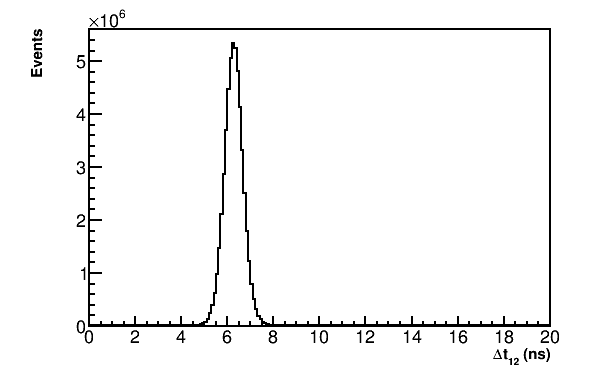
\includegraphics[width=\textwidth]{triples_deltaT_Endgame}
        \caption{}
    \end{subfigure}% %you need this % here to add spacing between subfigures
    \hspace{1cm}
    \begin{subfigure}[]{0.45\textwidth}
        \centering
        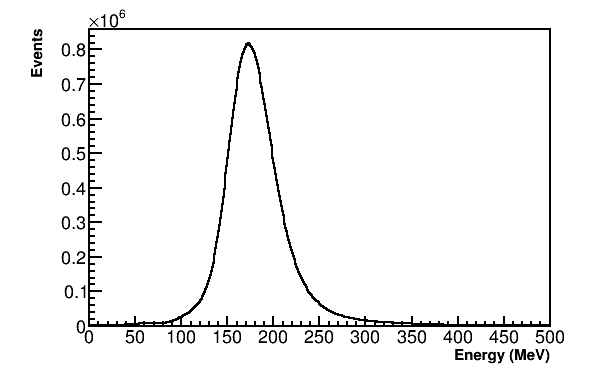
\includegraphics[width=\textwidth]{triples_Edep_Endgame}
        \caption{}
    \end{subfigure}
\caption[Lost muon $\Delta t$ and energy deposition distributions]{$\Delta t$ and energy deposition distributions for lost muons passing through adjacent calorimeters. A typical flight time is \ns{6.5} and energy deposition is 170 \MeV. Data from the Endgame dataset.}
\label{fig:lostmuondistributions}
\end{figure}


\begin{table}[]
\centering
\setlength\tabcolsep{10pt}
\renewcommand{\arraystretch}{1.2}
\begin{tabular*}{1\linewidth}{@{\extracolsep{\fill}}lc}
  \hline
    \multicolumn{2}{c}{\textbf{Lost Muon Cuts}} \\
  \hline\hline
    Parameter & Value or Range \\
  \hline
    Cluster size & $\leq$ 3 crystals \\
    Cluster energy fraction & $\geq$ 0.8 in main crystal \\
    Time of flight between adjacent calorimeters & $\SI{5}{ns} \leq \Delta t_{12, 23} \leq \SI{7.5}{ns}$ \\
    Energy deposition & $\SI{100}{\MeV} \leq E_{1,2,3} \leq \SI{250}{\MeV}$ \\
    Time of flight between separated calorimeters & $\Delta t_{13} \leq \SI{14.4}{ns}$ \\
  \hline 
\end{tabular*}
\caption[Lost muon cuts]{Lost muon selection cuts. In a triple coincidence the subscripts of 1, 2, and 3 correspond to the three calorimeters hit clockwise around the ring.}
\label{tab:lostmuoncuts}
\end{table}



The cuts used for the lost muon selection are given in \tabref{tab:lostmuoncuts}. Only those triple coincidences where every cluster consists of three or less crystals hit, with 80\% of the energy deposited in one crystal, are included. $\Delta t$ and energy deposition ranges are taken as $\SI{5}{ns} \leq \Delta t_{12, 23} \leq \SI{7.5}{ns}$ and $\SI{100}{\MeV} \leq E_{1,2,3} \leq \SI{250}{\MeV}$, where these ranges come from inspection of \figref{fig:lostmuondistributions}. The \DT distribution as a function of time in-fill is shown in \figref{fig:deltaT12_AccSub}. By examining this distribution in the range $\SI{2}{ns} \leq \Delta t_{12} \leq \SI{4}{ns}$, and averaging the contained counts, an approximation for the accidental background can be determined and subtracted off the triples spectrum. The accidental background typically comes from either double coincidences and a real positron hit, or a particle shower induced by an incident positron which hits a coincident calorimeter. 


\begin{figure}[]
\centering
        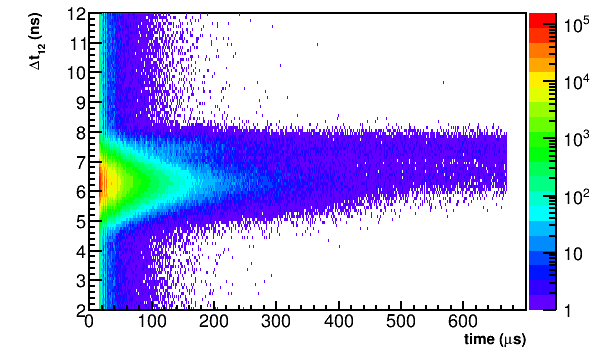
\includegraphics[width=0.9\textwidth]{deltaT12_beforeAccSubtraction_Endgame}
        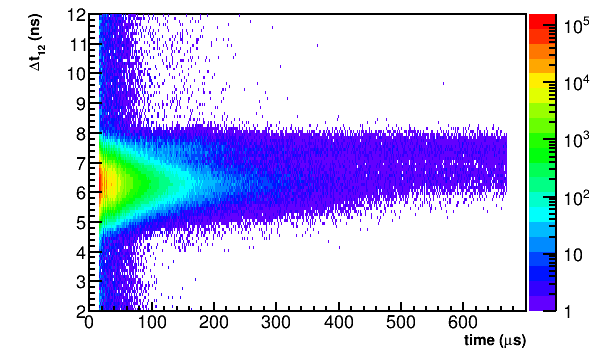
\includegraphics[width=0.9\textwidth]{deltaT12_afterAccSubtraction_Endgame}
\caption[Lost muon \DT distribution as a function of time in-fill]{\DT distribution as a function of time in-fill before (top) and after (bottom) accidental background subtraction. Note the log scale and the cahnge in colors at the far left of the bottom plot. Lost muons have a \DT distribution centered at \ns{6.5}. The accidental background can be seen as counts out at $\Delta t$'s far from the center of the distribution. Color striations in the core of the distribution correspond to CBO periods. There are two bands of hits that do not fall off as severely with time as the lost muons do. The band contained between 7 and \ns{8} corresponds to deuterons, while the band contained between 6 and \ns{7} corresponds to protons. Data from the Endgame dataset.}
\label{fig:deltaT12_AccSub}
\end{figure}


Also shown in \figref{fig:deltaT12_AccSub} are two bands of stable beam contaminants corresponding to stored dueterons and protons. These particles have different times of flights between calorimeters due to their larger masses. By looking at the $\Delta t_{13}$ distribution for times greater than \mus{300}, the deuteron population is easily isolated, \figref{fig:deuteronPop}. While the deuteron population is mostly removed by the \DT cut, an additional cut of $\Delta t_{13} \leq \SI{14.4}{ns}$ helps remove any remaining deuteron contaminants. The proton population, due to it's nearness to the real lost muon population, is harder to remove. The simplest solution is to simply cut on the negative side of the \DT or $\Delta t_{13}$ distribution. See \secref{sub:lostmuonserror} for the results using this additional cut, and the systematic error on R. It was found that the proton contamination makes almost no difference to the fitted value of R. The default then is to use the previously specified cut ranges in order to increase the amount of statistics in the lost muons distribution with which to fit. \figref{fig:finalDT12Dist} shows the final \DT distribution with cuts as a function of time in-fill for selected lost muons.


\begin{figure}[]
    \centering
    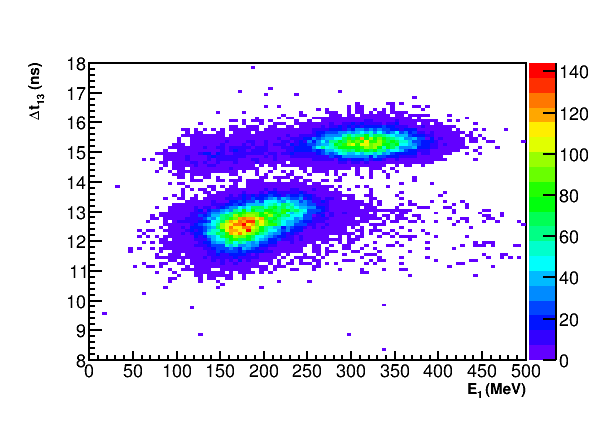
\includegraphics[width=.8\textwidth]{deuteron_Population_Endgame}
    \caption[Deuteron population at late times]{$\Delta t_{13}$ distribution as a function of energy for times greater than \mus{300}. The lost muons can be seen as a blob centered at 170 \MeV and a smaller $\Delta t_{13}$, while the deuterons can be seen at a higher $\Delta t_{13}$. While the deuterons have a preferentially larger energy deposition, they can be seen to extend to low energies. Data from the Endgame dataset.}
    \label{fig:deuteronPop}
\end{figure}


\begin{figure}[]
    \centering
    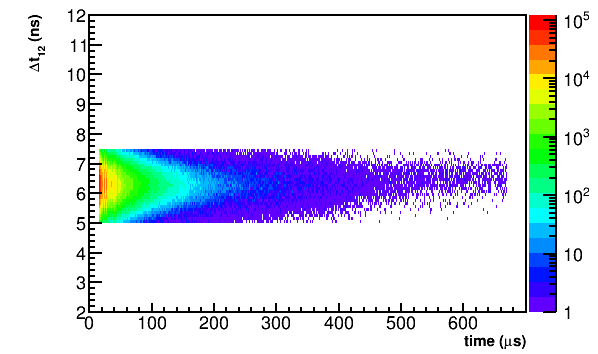
\includegraphics[width=.8\textwidth]{deltaT12_timeInFill_finalCuts_Endgame}
    \caption[Final \DT distribution for selected lost muons]{Final \DT distribution for selected lost muons as a function of time in-fill. Data from the Endgame dataset.}
    \label{fig:finalDT12Dist}
\end{figure}





\begin{figure}[]
    \centering
    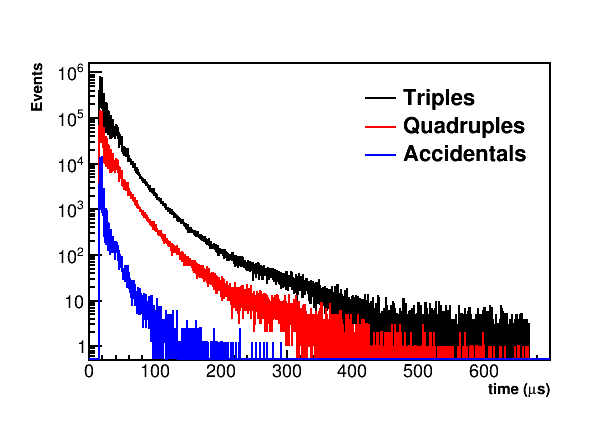
\includegraphics[width=.8\textwidth]{Triples_vs_all_Endgame}
    \caption[]{Data from the Endgame dataset.}
    \label{fig:}
\end{figure}



\begin{figure}[]
    \centering
    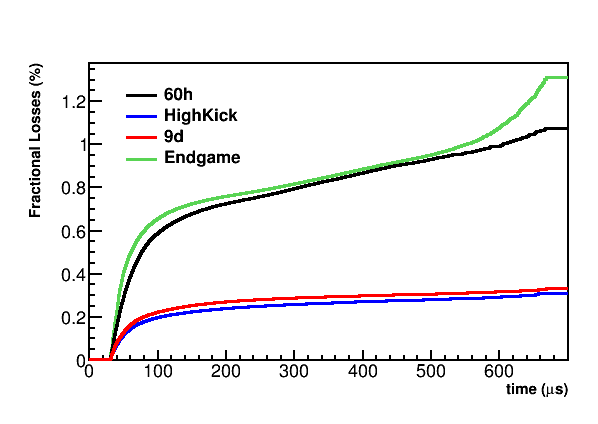
\includegraphics[width=.8\textwidth]{fractionalLosses_dataset_comparison}
    \caption[]{\textbf{update picture as necessary}}
    \label{fig:}
\end{figure}



Once we have the lost muons distribution we need to include them in the fit function somehow...




-go through procedure for accidental background subtraction

-include here the construction of the lost muon histogram and then go into the fitting stuff
-look through 60h report for things I should mention - things like arbitraty 10 to the 10 factor and such

-decide which plots to put in

\cite{lostmuonspaper}
\cite{lostmuonsDenverTalk}

- maybe cite Kevin's note too

    % \Lambda(t) = 1 - \boldsymbol{\kappa_{loss}} \int_{0}^{t} L(t')e^{(t'/\gamma\tau_{\mu})} dt'


-reference lost muons systematics error section 






\subsection{Fit code/parameter specifics}


when all is said and done there is X fit parameters used in the fit, on the order of 20 depending on dataset...

-a root macro is used to fit the data, and then to make plots


Fit is from \mus{30.2}--\mus{650}, corresponding to 4154 bins.


\begin{table}[]
\centering
\setlength\tabcolsep{10pt}
\renewcommand{\arraystretch}{1.2}
\begin{tabular*}{.8\linewidth}{@{\extracolsep{\fill}}lc}
  \hline
    \multicolumn{2}{c}{\textbf{Fit Procedure Parameters}} \\
  \hline\hline
    Parameter & Value \\
  \hline
    Fit start time & \mus{30.2} \\
    Fit end time & \mus{650} \\
  \hline 
\end{tabular*}
\caption[]{\textbf{fill this table out more once I've gone through the various parts}}
\label{tab:fitprocedureparameters}
\end{table}





\section{Fit results}

Fit results are blah from a single random seed ... 

remind that R is blinded
mention that a different blinding is used for 60h
mention that R will be slightly different between datasets due to field conditions 

Include here a table of the fit parameters and p value and such, per dataset, include 9d numbers from Elba for now


	\begin{table}[]
	\centering
	\setlength\tabcolsep{10pt}
	\renewcommand{\arraystretch}{1.2}
	\begin{tabular*}{.85\linewidth}{@{\extracolsep{\fill}}lcccc}
	  \hline
	  	\multicolumn{5}{c}{\textbf{9d Fit Results}} \\
	  \hline\hline
	  	& \multicolumn{2}{c}{T Method} & \multicolumn{2}{c}{R Method} \\
	  \hline\hline
	    $\chi^{2}$/NDF & \multicolumn{2}{c}{$4444/4444$} & \multicolumn{2}{c}{$4444/4444$} \\
	  	p value        & \multicolumn{2}{c}{$0.5$} & \multicolumn{2}{c}{$0.5$}  \\
	  \hline\hline
	  	Parameter & Value & Error & Value & Error \\
	  \hline
		$N_{0}$    			  		&  $\SI{3.452e+06}{}$ & $\SI{271.5}{}$ & $\SI{3.452e+06}{}$ & $\SI{271.5}{}$ \\
		$\tau$ (\mus{})   	    	&  $\SI{64.44}{}$ & $\SI{0.0038}{}$ & $\SI{64.44}{}$ & $\SI{0.0038}{}$ \\
		$A$    			 	  		&  $\SI{0.3704}{}$ & $\SI{4.396e-05}{}$ & $\SI{0.3704}{}$ & $\SI{4.396e-05}{}$ \\
		$R$ (ppm, blinded) 	  		&  $\SI{-20.450}{}$ & $\SI{1.311}{}$ & $\SI{-20.450}{}$ & $\SI{1.311}{}$ \\
		$\phi$   			  		&  $\SI{2.091}{}$ & $\SI{2.161e-4}{}$ & $\SI{2.091}{}$ & $\SI{2.161e-4}{}$ \\
		$\omega_{cbo}$ (rad/\mus{}) &  $\SI{0.367}{}$ & $\SI{6.936e-05}{}$ & $\SI{0.367}{}$ & $\SI{6.936e-05}{}$ \\
		$\tau_{cbo}$ (\mus{})       &  $\SI{178.9}{}$ & $\SI{14.7}{}$ & $\SI{178.9}{}$ & $\SI{14.7}{}$ \\
		$A_{cbo-N}$   	 	  		&  $\SI{0.00432}{}$ & $\SI{1.547e-4}{}$ & $\SI{0.00432}{}$ & $\SI{1.547e-4}{}$ \\
		$\phi_{cbo-N}$   	  		&  $\SI{-1.824}{}$ & $\SI{0.034}{}$ & $\SI{-1.824}{}$ & $\SI{0.034}{}$ \\
		$A_{2cbo-N}$   	 	  		&  $\SI{}{}$ & $\SI{}{}$ & $\SI{}{}$ & $\SI{}{}$ \\
		$\phi_{2cbo-N}$   	  		&  $\SI{}{}$ & $\SI{}{}$ & $\SI{}{}$ & $\SI{}{}$ \\
		$A_{cbo-A}$   	 	  		&  $\SI{6.075e-4}{}$ & $\SI{2.647e-4}{}$ & $\SI{6.075e-4}{}$ & $\SI{2.647e-4}{}$ \\
		$\phi_{cbo-A}$   	  		&  $\SI{-0.470}{}$ & $\SI{0.434}{}$ & $\SI{-0.470}{}$ & $\SI{0.434}{}$ \\
		$A_{cbo-\phi}$   	  		&  $\SI{2.586e-4}{}$ & $\SI{1.304e-4}{}$ & $\SI{2.586e-4}{}$ & $\SI{1.304e-4}{}$ \\
		$\phi_{cbo-\phi}$     		&  $\SI{-1.391}{}$ & $\SI{0.510}{}$ & $\SI{-1.391}{}$ & $\SI{0.510}{}$ \\
		$\kappa_{VW}$   	    	&  $\SI{2.309}{}$ & $\SI{0.00757}{}$ & $\SI{2.309}{}$ & $\SI{0.00757}{}$ \\
		$\tau_{VW}$ (\mus{})        &  $\SI{11.69}{}$ & $\SI{4.91}{}$ & $\SI{11.69}{}$ & $\SI{4.91}{}$ \\
		$A_{VW}$   	 		  		&  $\SI{0.018}{}$ & $\SI{0.019}{}$ & $\SI{0.018}{}$ & $\SI{0.019}{}$ \\
		$\phi_{VW}$   	  	  		&  $\SI{1.328}{}$ & $\SI{1.689}{}$ & $\SI{1.328}{}$ & $\SI{1.689}{}$ \\
		$\kappa_{loss}$   	    	&  $\SI{6.616}{}$ & $\SI{0.245}{}$ & $\SI{6.616}{}$ & $\SI{0.245}{}$ \\
	  \hline
	\end{tabular*}
	\caption[Fit parameter values versus dataset]{Fit parameters from ...\textbf{update numbers and such when results are final, including whether blinded or not, probably make R row bold, include errors and make it all look nice, do T method and R method side by side, state which parameters are fixed}}
	\label{tab:DatasetFitParametersValue}
	\end{table}




% \begin{landscape}
% \begin{table}[]
% \centering
% \small
% \setlength\tabcolsep{10pt}
% \renewcommand{\arraystretch}{1.2}
% \begin{tabular*}{1\linewidth}{@{\extracolsep{\fill}}lcccccccccccc}
%   \hline
%     \multicolumn{13}{c}{\textbf{Fit Parameter Values}} \\
%   \hline\hline
%     		  & \multicolumn{2}{c}{60h} & \multicolumn{2}{c}{HighKick} & \multicolumn{2}{c}{9d} & \multicolumn{2}{c}{LowKick} & \multicolumn{2}{c}{SuperLowKick} & \multicolumn{2}{c}{Endgame} \\
%   \hline
%     Parameter & T & R & T & R & T & R & T & R & T & R & T & R \\
%   \hline
%     $N_{0}$ &  &  &  &  &  &  &  &  &  &  &  &  \\
%     % $\tau_{\mu}$ (\mus{}) & 12 & 2.3389 & 2.9 & 81.8 & 5.12 & 7.7 \\                                        
%   \hline
% \end{tabular*}
% \caption[Fit parameter values versus dataset]{Fit parameters from ...\textbf{update numbers and such when results are final, including whether blinded or not, probably make R row bold, include errors and make it all look nice, do T method and R method side by side, state which parameters are fixed}}
% \label{tab:DatasetFitParametersValues}
% \end{table}
% \end{landscape}





In order to verify the integrity of the fit other checks are done ... 


\subsection{Per calorimeter fits}
\label{sub:per_calorimeter_fits}


\subsection{Fit start scans}

-include here the Kawall band equation as well as the full form


\subsection{Fit end scans}

\subsection{Fits to many random seeds}

\subsection{Energy threshold scan fits}

-should include here plots of A and N as well as R



\clearpage

-put here paramter values and all that for single seed fits to the individual datasets
-modulo plots
-maybe correlation matrix plots - or maybe those go into an appendix
-include FFT plots and pull plots 
-perhaps include or reference the average value of R










\section{Systematic errors}
\label{sec:Systematic Errors}



\begin{table}[]
\centering
\setlength\tabcolsep{10pt}
\renewcommand{\arraystretch}{1.2}
\begin{tabular*}{.8\linewidth}{@{\extracolsep{\fill}}lc}
  \hline
    \multicolumn{2}{c}{\textbf{\wa Measurement Uncertainties}} \\
  \hline\hline
    Source of uncertainty & E989 Goal (ppb) \\
  \hline
    Gain changes & 20 \\
    Pileup & 40 \\
    Lost muons & 20 \\
    CBO & 30 \\
    E field and pitch corrections & 30 \\
  \hline
    Quadrature sum & 70 \\
  \hline 
\end{tabular*}
\caption[Uncertainties in the precession frequency measurement]{Systematic errors in the precession frequency measurement. \textbf{fill this table out more once I've gone through the various parts}}
\label{tab:wauncertainties}
\end{table}




\subsection{Gain}
\label{sub:gainerror}


-talk about the equations here - slight reference to either detector section or reconstruction section in this chapter



\subsection{Pileup}
\label{sub:pileuperror}


For errors relating to the choice of SDT and SGT - the idea is this: Show the plots which show how the choices of SDT and SGT don't matter as long as the automatic pileup scaling is applied (shapes are the same) - this implies that the error due to these guys is contained within the pileup multiplier error, and can thus be ignored in favor of the latter - point back to pileup section when talking about this - I can also potentially if I have time do scans on these parameters and look at the effect on R

% https://gm2-docdb.fnal.gov/cgi-bin/private/RetrieveFile?docid=13963&filename=PileupScaleShadowTesting.pdf&version=1
% https://gm2-docdb.fnal.gov/cgi-bin/private/RetrieveFile?docid=14394&filename=PileupFormEtc.pdf&version=2


-pileup multiplier - amplitude
-pileup time shift - phase
-pileup energy scaling - phase


\subsection{CBO systematic errors}
\label{sub:cboerror}



\subsection{Lost muons}
\label{sub:lostmuonserror}
-also Sudeshna's talk in the Elba collaboration meeting - this probably just for the systematic error

-negative side cut
-chart with different fits
-if different cuts are made then k loss simply compensates and the fit is basically the same


- a systematic error comes from the fact that muons are lost preferentially at earlier times (changing over the course of a fill)
-if lost muons originate from different points in the beam line, then they will have precessed a different amount leading to a different phase





\begin{figure}[]
    \centering
    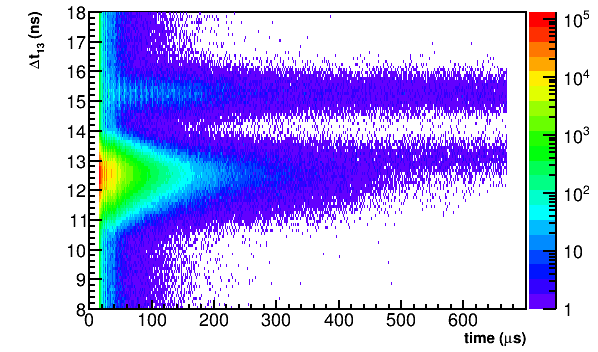
\includegraphics[width=.8\textwidth]{deltaT13_timeInFill_noCuts_Endgame}
    \caption[]{\textbf{update picture as necessary}}
    \label{fig:}
\end{figure}


\subsection{gm2 period guess and muon lifetime - Ratio construction parameters}
\label{sub:TimeShiftingParameters}



\subsection{Fits to bunch number}


\subsection{Binning}



\subsection{Systematic error summary}

-include here a big table (with each of the individual errors making up say pileup and the like) of all systematic errors



\cleardoublepage




% \begin{figure}[]
%     \centering
%     \includegraphics[width=.8\textwidth]{}
%     \caption[]{\textbf{update picture as necessary}}
%     \label{fig:}
% \end{figure}

% \begin{figure}[]
% \centering
%     \begin{subfigure}[]{0.8\textwidth}
%         \centering
%         \includegraphics[width=\textwidth]{}
%         \caption{}
%     \end{subfigure}% %you need this % here to add spacing between subfigures
%     \vspace{1cm}
%     \begin{subfigure}[]{0.8\textwidth}
%         \centering
%         \includegraphics[width=\textwidth]{}
%         \caption{}
%     \end{subfigure}
% \caption[]{\textbf{update pictures as needed}}
% \label{fig:}
% \end{figure}

